\documentclass[aspectratio=169, 10pt, xcolor={table}]{beamer}

\usepackage[utf8]{inputenc}
\usepackage[T5]{fontenc}
\usepackage[vietnamese]{babel}
\usepackage{booktabs}
\usepackage{array}
\usepackage{tabularx}
\usepackage{tcolorbox}
\tcbuselibrary{skins}
\usepackage{tikz}
\usetikzlibrary{positioning, arrows.meta, calc, backgrounds}

% ============================================================
% BẢNG MÀU
% ============================================================
\definecolor{navy}{HTML}{0B2545}
\definecolor{brand}{HTML}{2A78D6}
\definecolor{brandSoft}{HTML}{E8F1FC}
\definecolor{accent}{HTML}{EB6834}
\definecolor{accentSoft}{HTML}{FDEEE7}
\definecolor{okGreen}{HTML}{0E8A4F}
\definecolor{okSoft}{HTML}{E6F4EC}
\definecolor{warnAmber}{HTML}{B7791F}
\definecolor{warnSoft}{HTML}{FDF4E3}
\definecolor{badRed}{HTML}{C53030}
\definecolor{badSoft}{HTML}{FCEBEB}
\definecolor{ink}{HTML}{1F2933}
\definecolor{inkSoft}{HTML}{52606D}
\definecolor{line}{HTML}{D9E2EC}
\definecolor{paper}{HTML}{F5F7FA}

% ============================================================
% GIAO DIỆN BEAMER (tự thiết kế, không dùng theme có sẵn)
% ============================================================
\usefonttheme{professionalfonts}
\setbeamercolor{normal text}{fg=ink, bg=white}
\setbeamercolor{structure}{fg=brand}
\setbeamercolor{alerted text}{fg=accent}
\setbeamercolor{frametitle}{fg=navy}
\setbeamercolor{itemize item}{fg=brand}
\setbeamercolor{itemize subitem}{fg=inkSoft}
\setbeamercolor{enumerate item}{fg=brand}
\setbeamerfont{frametitle}{size=\Large, series=\bfseries}

\setbeamertemplate{navigation symbols}{}
\setbeamertemplate{itemize item}{\raisebox{0.15ex}{\tikz\fill[brand] (0,0) circle (0.55ex);}}
\setbeamertemplate{itemize subitem}{\raisebox{0.2ex}{\tikz\fill[inkSoft] (0,0) rectangle (0.8ex,0.8ex);}}
\setbeamertemplate{enumerate item}{%
    \tikz[baseline=(n.base)]\node[circle, fill=brand, text=white, inner sep=1.2pt, minimum size=1.35em,
        font=\scriptsize\bfseries] (n) {\insertenumlabel};}
\setlength{\leftmargini}{1.4em}

% Tiêu đề trang: nhãn mục nhỏ + tiêu đề lớn + vạch nhấn
\setbeamersize{text margin left=0.75cm, text margin right=0.6cm}
\setbeamertemplate{frametitle}{%
    \vspace*{0.12cm}%
    \begin{minipage}{\textwidth}
        {\tiny\color{inkSoft}\MakeUppercase{\insertsectionhead}}\par
        {\usebeamerfont{frametitle}\color{navy}\insertframetitle}\par\vspace{1pt}
        \tikz\fill[brand] (0,0) rectangle (1.4cm,2pt);\tikz\fill[accent] (0,0) rectangle (0.5cm,2pt);
    \end{minipage}%
    \vspace*{-0.25cm}%
}

% Chân trang mảnh: tên báo cáo + số trang
\setbeamertemplate{footline}{%
    \begin{tikzpicture}[remember picture, overlay]
        \draw[line, line width=0.4pt] ([xshift=0.6cm, yshift=0.55cm]current page.south west)
            -- ([xshift=-0.6cm, yshift=0.55cm]current page.south east);
        \node[anchor=south west, font=\tiny, text=inkSoft]
            at ([xshift=0.6cm, yshift=0.18cm]current page.south west)
            {Campus Network SDN \& SD-WAN \quad$\cdot$\quad Báo cáo cuối kỳ Dự án Công nghệ thông tin};
        \node[anchor=south east, font=\tiny\bfseries, text=brand]
            at ([xshift=-0.6cm, yshift=0.18cm]current page.south east)
            {\insertframenumber\,/\,\inserttotalframenumber};
    \end{tikzpicture}%
}

% Dải màu bên trái mỗi trang
\setbeamertemplate{background}{%
    \begin{tikzpicture}[remember picture, overlay]
        \fill[navy] (current page.north west) rectangle ([xshift=0.18cm]current page.south west);
    \end{tikzpicture}%
}

% Trang chuyển mục
\AtBeginSection[]{%
    {\setbeamertemplate{footline}{}
    \begin{frame}[plain, noframenumbering]
        \begin{tikzpicture}[remember picture, overlay]
            \fill[navy] (current page.south west) rectangle (current page.north east);
            \fill[brand] ([yshift=-0.2cm]current page.west) rectangle ([xshift=2.2cm, yshift=0.2cm]current page.west);
            \fill[accent] ([xshift=2.2cm, yshift=-0.2cm]current page.west) rectangle ([xshift=3.0cm, yshift=0.2cm]current page.west);
            \node[anchor=west, text=white!60!navy, font=\Huge\bfseries]
                at ([xshift=1.2cm, yshift=1.5cm]current page.west) {\scalebox{2.2}{0\insertsectionnumber}};
            \node[anchor=west, text=white, font=\huge\bfseries, text width=11cm]
                at ([xshift=3.5cm]current page.west) {\insertsectionhead};
        \end{tikzpicture}
    \end{frame}}
}

% ============================================================
% THÀNH PHẦN: thẻ nội dung, nhãn trạng thái, ô số liệu, ảnh
% ============================================================
\newtcolorbox{card}[2][brand]{enhanced, colback=white, colframe=line, boxrule=0.5pt, arc=3pt,
    left=6pt, right=6pt, top=4pt, bottom=4pt,
    borderline north={2pt}{0pt}{#1},
    title={\color{#1}\bfseries #2}, coltitle=navy, colbacktitle=white,
    attach title to upper, after title={\par\vspace{2pt}}, fontupper=\small}
\newtcolorbox{softcard}[1][brandSoft]{enhanced, colback=#1, frame hidden, arc=3pt,
    left=6pt, right=6pt, top=4pt, bottom=4pt, fontupper=\small}

\newcommand{\pill}[3]{\tcbox[on line, colback=#2, colframe=#2, arc=6pt, boxrule=0pt,
    left=4pt, right=4pt, top=1pt, bottom=1pt, fontupper=\scriptsize\bfseries\color{#1}]{#3}}
\newcommand{\done}{\pill{okGreen}{okSoft}{Hoàn thành}}
\newcommand{\pass}{\pill{okGreen}{okSoft}{Đạt}}
\newcommand{\partly}{\pill{warnAmber}{warnSoft}{Một phần}}

% Ô số liệu lớn
\newcommand{\stat}[3]{% màu, số, chú thích
    \begin{tcolorbox}[enhanced, colback=white, colframe=line, boxrule=0.5pt, arc=3pt,
        borderline west={3pt}{0pt}{#1}, left=8pt, top=3pt, bottom=3pt]
        {\Large\bfseries\color{#1}#2}\par
        {\raggedright\scriptsize\color{inkSoft}#3\par}
    \end{tcolorbox}}

% Ảnh chụp màn hình có viền mảnh và chú thích
\newcommand{\shot}[2][width=\linewidth]{{\setlength{\fboxsep}{0pt}\setlength{\fboxrule}{0.4pt}%
    \fcolorbox{line}{white}{\includegraphics[#1]{#2}}}}
\newcommand{\capt}[1]{{\par\vspace{1pt}\scriptsize\color{inkSoft}#1\par}}

\newcolumntype{Y}{>{\raggedright\arraybackslash}X}
\newcolumntype{L}[1]{>{\raggedright\arraybackslash}p{#1}}
\renewcommand{\arraystretch}{1.25}
\newcommand{\hd}[1]{\textcolor{navy}{\textbf{#1}}}
\newcommand{\compactlist}{\setlength{\itemsep}{1pt}\setlength{\parskip}{0pt}}

% Ảnh riêng của slide nằm trong image/, ảnh dùng chung lấy từ báo cáo cuối kỳ
\graphicspath{{image/}{../cuoi-ky/image/}}

\title{XÂY DỰNG CAMPUS NETWORK\\SỬ DỤNG SDN VÀ SD-WAN}
\subtitle{Báo cáo cuối kỳ -- Dự án Công nghệ thông tin}
\author{Trần Hữu Nhân -- 52300235 \quad$\cdot$\quad Nguyễn Nhật Hào -- 52300198}
\institute{Khoa Công nghệ Thông tin -- Trường Đại học Tôn Đức Thắng}
\date{11/2026}

\begin{document}

% ============================================================
% TRANG BÌA
% ============================================================
{\setbeamertemplate{background}{}\setbeamertemplate{footline}{}
\begin{frame}[plain, noframenumbering]
    \begin{tikzpicture}[remember picture, overlay]
        \fill[navy] (current page.north west) rectangle ([xshift=9.6cm]current page.south west);
        \fill[brand] ([xshift=9.6cm]current page.north west) rectangle ([xshift=9.85cm]current page.south west);
        \fill[accent] ([xshift=9.6cm, yshift=-2.2cm]current page.north west) rectangle ([xshift=9.85cm, yshift=-3.2cm]current page.north west);
        % mô típ mạng
        \begin{scope}[shift={([xshift=12.9cm, yshift=-0.9cm]current page.west)}, every node/.style={circle, inner sep=0pt}]
            \foreach \p/\n in {(0,1.5)/a, (-1.4,0.4)/b, (1.4,0.4)/c, (-0.9,-1.2)/d, (0.9,-1.2)/e, (0,0)/f}
                \node[fill=brand, minimum size=7pt] (\n) at \p {};
            \foreach \u/\v in {a/f, b/f, c/f, d/f, e/f, a/b, a/c, b/d, c/e, d/e}
                \draw[brand!45, line width=1pt] (\u) -- (\v);
            \node[fill=accent, minimum size=11pt] at (f) {};
        \end{scope}
        \node[anchor=north, inner sep=0pt] at ([xshift=12.9cm, yshift=-0.75cm]current page.north west)
            {
\includegraphics[width=1.9cm]{logo-tdtu.jpg}};
        \node[anchor=north west, text=white!70!navy, font=\scriptsize\bfseries, align=left]
            at ([xshift=0.9cm, yshift=-0.8cm]current page.north west)
            {TRƯỜNG ĐẠI HỌC TÔN ĐỨC THẮNG \,·\, KHOA CÔNG NGHỆ THÔNG TIN\\[2pt]DỰ ÁN CÔNG NGHỆ THÔNG TIN};
        \node[anchor=south west, text=white, font=\Large\bfseries, text width=8.4cm, align=left]
            at ([xshift=0.9cm, yshift=0.15cm]current page.west) {XÂY DỰNG CAMPUS NETWORK\\SỬ DỤNG SDN VÀ SD-WAN};
        \node[anchor=north west, text=white!80!brand, font=\small\itshape, text width=8.4cm, align=left]
            at ([xshift=0.9cm, yshift=-0.05cm]current page.west) {Implementation of an SDN- and SD-WAN-Based Campus Network};
        \node[anchor=west, fill=accent, text=white, font=\footnotesize\bfseries, rounded corners=2pt, inner sep=4pt]
            at ([xshift=0.9cm, yshift=-1.3cm]current page.west) {Báo cáo cuối kỳ \,·\, Mạng máy tính và truyền thông dữ liệu};
        \node[anchor=south west, text=white, font=\footnotesize, align=left]
            at ([xshift=0.9cm, yshift=0.6cm]current page.south west)
            {{\color{white!70!navy}Người hướng dẫn:} \textbf{ThS. Lê Viết Thanh}\\[3pt]
             {\color{white!70!navy}Sinh viên thực hiện:}\\
             \textbf{Trần Hữu Nhân} -- 52300235\\\textbf{Nguyễn Nhật Hào} -- 52300198};
        \node[anchor=south, text=inkSoft, font=\scriptsize]
            at ([xshift=12.9cm, yshift=0.6cm]current page.south west) {TP. Hồ Chí Minh, tháng 11 năm 2026};
    \end{tikzpicture}
\end{frame}}

\begin{frame}{Nội dung trình bày}
    \vspace{0.15cm}
    \begin{columns}[T]
        \begin{column}{0.48\textwidth}
            \begin{softcard}\textbf{\color{brand}01}\quad \textbf{Tổng quan đề tài}\\
                {\scriptsize\color{inkSoft}Lý do, mục tiêu, phạm vi và phương pháp}\end{softcard}
            \begin{softcard}\textbf{\color{brand}02}\quad \textbf{Cơ sở lý thuyết}\\
                {\scriptsize\color{inkSoft}Mạng Campus phân cấp, SDN/OpenFlow, SD-WAN Viptela}\end{softcard}
            \begin{softcard}\textbf{\color{brand}03}\quad \textbf{Mô hình mạng Campus đề xuất}\\
                {\scriptsize\color{inkSoft}Kiến trúc, topology, IP/VLAN, thiết kế SDN, SD-WAN, bảo mật}\end{softcard}
        \end{column}
        \begin{column}{0.48\textwidth}
            \begin{softcard}\textbf{\color{brand}04}\quad \textbf{Triển khai và kiểm thử}\\
                {\scriptsize\color{inkSoft}Campus chính, SDN, SD-WAN, Internet, dịch vụ, NetOps Bot}\end{softcard}
            \begin{softcard}\textbf{\color{brand}05}\quad \textbf{Đánh giá và kết luận}\\
                {\scriptsize\color{inkSoft}30 kịch bản, 7 nhóm tiêu chí đề cương, hạn chế, hướng phát triển}\end{softcard}
            \begin{softcard}[accentSoft]\scriptsize
                Số liệu trong slide lấy từ báo cáo cuối kỳ; mọi kết quả đều đo trên hệ thống đang chạy
                bằng script tự động và có thể chạy lại.\end{softcard}
        \end{column}
    \end{columns}
\end{frame}

% ============================================================
% 01. TỔNG QUAN ĐỀ TÀI
% ============================================================
\section{Tổng quan đề tài}

\begin{frame}{Lý do chọn đề tài}
    \begin{columns}[T]
        \begin{column}{0.48\textwidth}
            \begin{card}[badRed]{Mạng Campus truyền thống}
                \footnotesize
                \begin{itemize}\compactlist
                    \item Cấu hình \textbf{trực tiếp trên từng thiết bị}: mỗi switch tự học địa chỉ, tự chạy STP; mỗi router khai báo định tuyến riêng.
                    \item Đổi VLAN, áp chính sách, xử lý sự cố phải làm trên \textbf{nhiều thiết bị} $\Rightarrow$ dễ sai lệch.
                    \item \textbf{Không có cái nhìn toàn cục} về trạng thái lớp 2 và lưu lượng.
                    \item WAN liên cơ sở phụ thuộc \textbf{một đường thuê riêng}, không tự chọn đường theo chất lượng, tốn kém khi dự phòng.
                \end{itemize}
            \end{card}
        \end{column}
        \begin{column}{0.48\textwidth}
            \begin{card}{SDN -- cho mạng nội bộ}
                \footnotesize
                Tách mặt phẳng điều khiển khỏi switch: một \textbf{Controller} lập trình, giám sát và áp chính sách tập trung.
            \end{card}
            \begin{card}[accent]{SD-WAN -- cho kết nối liên cơ sở}
                \footnotesize
                Overlay mã hóa trên \textbf{nhiều đường truyền} (Internet, MPLS), quản lý tập trung, chọn đường theo chất lượng thực tế.
            \end{card}
        \end{column}
    \end{columns}
    \vspace{0.05cm}
    \begin{softcard}[okSoft]\footnotesize
        \textbf{\color{okGreen}Đề tài:} kết hợp kiến trúc Campus phân cấp với SDN và SD-WAN cho một trường đại học đa cơ sở,
        \textbf{hiện thực và kiểm chứng} trên một mô hình cụ thể.
    \end{softcard}
\end{frame}

\begin{frame}{Nội dung đề cương và mức độ hiện thực}
    \begin{card}{Đề tài số 2 -- nội dung đề cương \quad$\rightarrow$\quad hiện thực trong đồ án}
        \scriptsize
        \renewcommand{\arraystretch}{1.2}
        \begin{tabularx}{\linewidth}{@{}L{0.31\linewidth}Yc@{}}
            \hd{Nội dung} & \hd{Hiện thực} & \hd{Trạng thái} \\
            \midrule
            Mô hình Core -- Distribution -- Access & Site 100: 2 Core IOL (VRRP, OSPF), 2 Distribution + 4 Access (OVS) & \done \\
            VLAN theo khoa, phòng máy, hành chính & VLAN 10 CNTT, 20 Toán--TK, 30 Luật, 40 Hành chính, 90 Server Farm & \done \\
            SDN Controller quản lý switch & Ryu + OpenFlow 1.3 điều khiển 6 OVS, tự phục hồi, SDN Console & \done \\
            SD-WAN nối Campus chính với cơ sở phụ & Viptela: 10 vEdge, 5 site, Internet + MPLS, BFD/AAR, chính sách vSmart & \done \\
            STP/RSTP, OSPF, DHCP, ACL, dự phòng liên kết & Rapid-PVST+, OSPF Area 0, DHCP qua relay, ACL tường lửa, Po10/VRRP/FW HA & \done \\
            \midrule
            \textit{Bổ sung ngoài đề cương} & Internet tại chỗ (DIA) có dự phòng, DNS/Web/Mail/Syslog, cảnh báo email, Campus NetOps Bot & \done \\
        \end{tabularx}
    \end{card}
\end{frame}

\begin{frame}{Mục tiêu, phạm vi và phương pháp}
    \begin{columns}[T]
        \begin{column}{0.235\textwidth}\stat{brand}{74 node}{107 phân đoạn mạng trên một lab EVE-NG}\end{column}
        \begin{column}{0.235\textwidth}\stat{accent}{6 site}{Campus chính, 3 cơ sở phụ, Site 500, Site 900 + 2 nhà cung cấp}\end{column}
        \begin{column}{0.235\textwidth}\stat{okGreen}{6 OVS}{do một Controller Ryu điều khiển qua OpenFlow 1.3}\end{column}
        \begin{column}{0.235\textwidth}\stat{brand}{10 vEdge}{112 đường hầm IPsec trên 2 transport}\end{column}
    \end{columns}
    \vspace{-0.1cm}
    \begin{columns}[T]
        \begin{column}{0.49\textwidth}
            \begin{card}{Mục tiêu}
                \scriptsize
                \begin{itemize}\compactlist
                    \item Campus chính 3 tầng: VRRP, OSPF, tường lửa Active/Standby, DMZ, Server Farm.
                    \item Chi nhánh rút gọn \textbf{Firewall-as-Core} cho Cần Thơ, Đà Nẵng, Nha Trang.
                    \item Ứng dụng Ryu điều khiển toàn bộ lớp 2 và \textbf{đo 5 tiêu chí định lượng}.
                    \item SD-WAN Viptela: BGP underlay, PKI, SLA, AAR, lọc tập trung, cảnh báo.
                    \item Internet tại chỗ có dự phòng; dịch vụ dùng chung; bảo mật nhiều lớp.
                \end{itemize}
            \end{card}
        \end{column}
        \begin{column}{0.49\textwidth}
            \begin{card}[accent]{Phạm vi và phương pháp}
                \scriptsize
                \begin{itemize}\compactlist
                    \item \textbf{Hybrid SDN:} SDN cho Distribution/Access; Core và tường lửa giữ cơ chế truyền thống.
                    \item Triển khai \textbf{từ dưới lên}: underlay $\rightarrow$ controller $\rightarrow$ hạ tầng $\rightarrow$ dịch vụ $\rightarrow$ chính sách.
                    \item Kiểm thử, chẩn đoán \textbf{theo lớp}; kết luận dựa trên \texttt{show}, thống kê, bắt gói.
                    \item Cấu hình mọi thiết bị quản lý bằng Git; phép đo tự động hóa bằng script.
                    \item Ngoài phạm vi: mạng không dây, 802.1X.
                \end{itemize}
            \end{card}
        \end{column}
    \end{columns}
\end{frame}

% ============================================================
% 02. CƠ SỞ LÝ THUYẾT
% ============================================================
\section{Cơ sở lý thuyết}

\begin{frame}{Mạng Campus phân cấp và các cơ chế truyền thống}
    \begin{columns}[c]
        \begin{column}{0.44\textwidth}
            \centering
            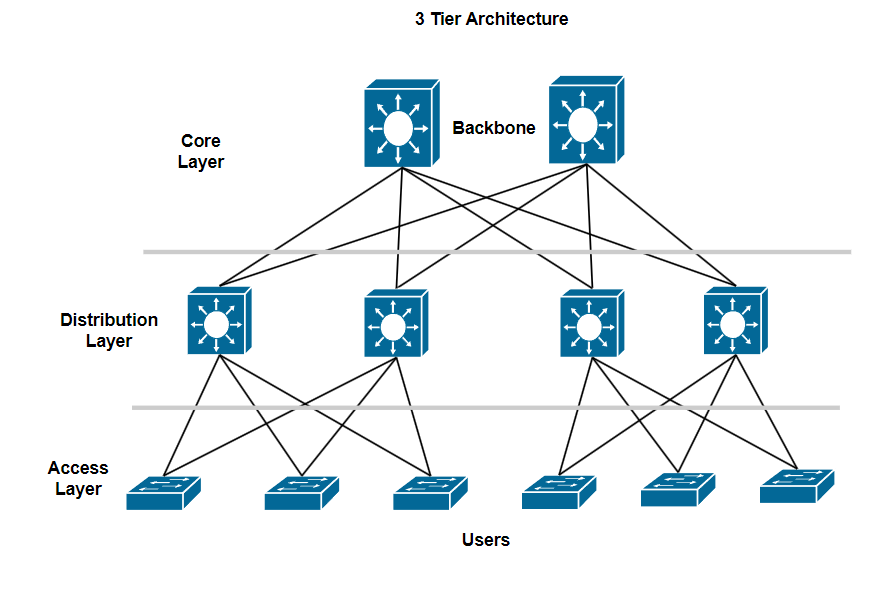
\includegraphics[width=\linewidth]{mohinh.png}
            \capt{Mô hình phân cấp Core -- Distribution -- Access}
        \end{column}
        \begin{column}{0.54\textwidth}
            \begin{card}{Ba tầng, ba vai trò}
                \scriptsize
                \begin{itemize}\compactlist
                    \item \textbf{Access:} kết nối người dùng, gán VLAN theo cổng.
                    \item \textbf{Distribution:} gom Access, áp chính sách, dự phòng đường lên.
                    \item \textbf{Core:} chuyển mạch tốc độ cao, định tuyến liên VLAN, nối biên.
                \end{itemize}
            \end{card}
            \begin{card}[accent]{Cơ chế nền tảng dùng trong đề tài}
                \scriptsize
                \renewcommand{\arraystretch}{1.1}
                \begin{tabularx}{\linewidth}{@{}L{0.33\linewidth}Y@{}}
                    VLAN, trunk 802.1Q & Phân đoạn theo khoa/khối, mỗi VLAN một subnet \\
                    Rapid-PVST+, LACP & Chống vòng lớp 2, gộp liên kết giữa hai Core \\
                    VRRP & Gateway dự phòng cho từng VLAN \\
                    OSPF, BGP & Định tuyến nội bộ; định tuyến với nhà cung cấp \\
                    IP SLA + track & Tuyến tĩnh dự phòng theo trạng thái đường đi \\
                    ASA, DMZ & Tường lửa trạng thái, vùng dịch vụ công bố \\
                \end{tabularx}
            \end{card}
        \end{column}
    \end{columns}
\end{frame}

\begin{frame}{Công nghệ SDN và OpenFlow 1.3}
    \begin{columns}[c]
        \begin{column}{0.42\textwidth}
            \centering
            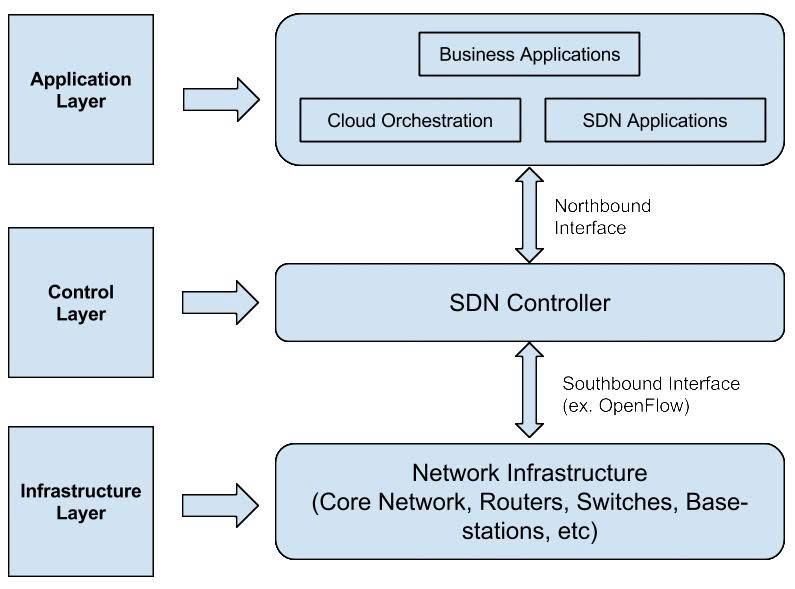
\includegraphics[width=\linewidth]{SDN_ARCHITECTURE.jpg}
            \capt{Kiến trúc SDN ba lớp}
        \end{column}
        \begin{column}{0.56\textwidth}
            \begin{card}{Nguyên lý}
                \scriptsize
                \begin{itemize}\compactlist
                    \item Tách \textbf{mặt phẳng điều khiển} (Controller) khỏi \textbf{mặt phẳng dữ liệu} (switch).
                    \item \textbf{OpenFlow 1.3} (southbound): switch khớp gói theo bảng flow (match $\rightarrow$ action); gói không khớp gửi \texttt{Packet-In} lên Controller, Controller trả \texttt{Flow-Mod}.
                    \item \textbf{REST API} (northbound) cho ứng dụng giám sát, tự động hóa.
                \end{itemize}
            \end{card}
            \begin{card}[accent]{Thành phần sử dụng}
                \scriptsize
                \begin{itemize}\compactlist
                    \item \textbf{Open vSwitch} -- switch ảo hỗ trợ OpenFlow, nhiều bảng flow.
                    \item \textbf{Ryu} -- framework Controller bằng Python; nhóm tự viết ứng dụng.
                    \item \textbf{ONOS} -- đã thử để quan sát topology, sau đó tắt vì chiếm CPU.
                \end{itemize}
            \end{card}
            \begin{softcard}\scriptsize
                \textbf{Ưu:} lập trình được, quan sát toàn cục, chính sách tập trung.\quad
                \textbf{Nhược:} Controller là điểm trọng yếu; kênh điều khiển in-band phức tạp.
            \end{softcard}
        \end{column}
    \end{columns}
\end{frame}

\begin{frame}{Công nghệ SD-WAN -- kiến trúc Cisco Viptela}
    \begin{columns}[c]
        \begin{column}{0.47\textwidth}
            \centering
            \begin{tikzpicture}[font=\scriptsize,
                box/.style={draw=line, fill=white, rounded corners=3pt, align=center, minimum height=0.8cm, text width=1.9cm},
                ctl/.style={box, draw=brand, fill=brandSoft},
                edge/.style={box, draw=accent, fill=accentSoft, text width=1.6cm},
                tr/.style={box, fill=paper, text width=2.1cm, minimum height=0.6cm}]
                \node[ctl] (vm) at (-2.3,3.3) {\textbf{vManage}\\quản trị, giám sát};
                \node[ctl] (vs) at (0,3.3) {\textbf{vSmart}\\điều khiển, OMP};
                \node[ctl] (vb) at (2.3,3.3) {\textbf{vBond}\\điều phối, xác thực};
                \node[tr] (in) at (-1.4,1.55) {Internet\\\texttt{biz-internet}};
                \node[tr] (mp) at (1.4,1.55) {MPLS\\\texttt{mpls}};
                \node[edge] (e1) at (-2.6,-0.1) {\textbf{vEdge}\\Site A};
                \node[edge] (e2) at (2.6,-0.1) {\textbf{vEdge}\\Site B};
                \draw[brand, dashed, -{Stealth[length=3pt]}] (vs) -- (e1.north east);
                \draw[brand, dashed, -{Stealth[length=3pt]}] (vs) -- (e2.north west);
                \draw[accent, line width=1pt] (e1) -- (in) -- (e2);
                \draw[okGreen, line width=1pt] (e1) -- (mp) -- (e2);
                \draw[inkSoft, line width=1.6pt, {Stealth[length=4pt]}-{Stealth[length=4pt]}] (e1) -- node[below, text=inkSoft]{đường hầm IPsec + BFD} (e2);
                \node[text=brand, font=\tiny] at (0,2.45) {DTLS / OMP (dashed)};
            \end{tikzpicture}
        \end{column}
        \begin{column}{0.51\textwidth}
            \begin{card}{Bốn thành phần -- ba mặt phẳng}
                \scriptsize
                \begin{itemize}\compactlist
                    \item \textbf{vManage:} cấu hình, giám sát, alarm, REST API.
                    \item \textbf{vSmart:} phân phối tuyến và chính sách qua \textbf{OMP}.
                    \item \textbf{vBond:} xác thực thiết bị bằng chứng thư (PKI), giới thiệu controller.
                    \item \textbf{vEdge:} router biên, đầu cuối đường hầm IPsec.
                \end{itemize}
            \end{card}
            \begin{card}[accent]{Khái niệm chính}
                \scriptsize
                \begin{itemize}\compactlist
                    \item \textbf{TLOC + color:} điểm cuối đường hầm trên mỗi transport.
                    \item \textbf{BFD:} đo mất gói, trễ, jitter từng đường hầm $\Rightarrow$ phát hiện lỗi.
                    \item \textbf{VPN 0 / 1 / 512:} transport / dịch vụ / quản trị.
                    \item \textbf{Chính sách tập trung:} control policy, data policy, App-Aware Routing theo SLA.
                    \item \textbf{DIA:} ra Internet tại chỗ bằng NAT trên vEdge.
                \end{itemize}
            \end{card}
        \end{column}
    \end{columns}
\end{frame}

% ============================================================
% 03. MÔ HÌNH ĐỀ XUẤT
% ============================================================
\section{Mô hình mạng Campus đề xuất}

\begin{frame}{Bài toán và yêu cầu thiết kế}
    \begin{softcard}\footnotesize
        \textbf{\color{navy}Bối cảnh:} một trường đại học có \textbf{cơ sở chính} (3 khoa, khối Hành chính, toàn bộ dịch vụ dùng chung)
        và \textbf{3 cơ sở phụ} tại Cần Thơ, Đà Nẵng, Nha Trang -- mỗi cơ sở 2 khối nghiệp vụ, cần dùng dịch vụ tại cơ sở chính.
    \end{softcard}
    \vspace{-0.1cm}
    \begin{columns}[T]
        \begin{column}{0.56\textwidth}
            \begin{card}{Yêu cầu chức năng}
                \scriptsize
                \begin{itemize}\compactlist
                    \item \textbf{Kết nối:} mọi cơ sở dùng được dịch vụ chung; chi nhánh thông nhau theo chính sách.
                    \item \textbf{Phân đoạn:} mỗi khoa/khối một VLAN + subnet; tách máy chủ, DMZ, quản trị.
                    \item \textbf{Dịch vụ:} DHCP, DNS \texttt{campus.internal}, Web HTTPS, Mail, Syslog.
                    \item \textbf{SDN:} Controller quản lý toàn bộ lớp 2 Distribution/Access, chống vòng, REST API.
                    \item \textbf{SD-WAN:} xác thực chứng thư, overlay IPsec 2 transport, OMP, SLA/AAR.
                    \item \textbf{Bảo mật biên, Internet tại chỗ, giám sát và cảnh báo.}
                \end{itemize}
            \end{card}
        \end{column}
        \begin{column}{0.42\textwidth}
            \begin{card}[accent]{Yêu cầu phi chức năng}
                \scriptsize
                \begin{itemize}\compactlist
                    \item \textbf{Sẵn sàng:} không điểm lỗi đơn tại gateway (VRRP), lõi (2 Core, EtherChannel), biên (FW HA), WAN (2 Edge, 2 transport), lớp 2 (Access nối kép).
                    \item \textbf{Mở rộng:} địa chỉ theo mã site; site mới dùng lại khuôn chi nhánh.
                    \item \textbf{Quản trị:} vùng quản trị riêng, giao diện tập trung, nhật ký tập trung.
                    \item \textbf{Nhất quán:} mọi định danh ghi trong bảng quy hoạch.
                \end{itemize}
            \end{card}
        \end{column}
    \end{columns}
\end{frame}

\begin{frame}{Kiến trúc tổng thể -- topology logic mức site}
    \centering
    \begin{tikzpicture}[font=\scriptsize, >=Stealth,
        base/.style={rounded corners=3pt, align=center, line width=0.6pt},
        ctl/.style={base, draw=navy, fill=brandSoft, text width=7.6cm, minimum height=0.95cm},
        tr/.style={base, draw=inkSoft, fill=paper, text width=2.9cm, minimum height=0.75cm},
        hq/.style={base, draw=brand, fill=white, text width=7.0cm, minimum height=1.15cm, line width=1pt},
        br/.style={base, draw=okGreen, fill=okSoft, text width=3.05cm, minimum height=1.25cm}]
        \node[ctl] (s900) at (0,5.35) {\textbf{Site 900 -- Trung tâm điều khiển SD-WAN}\\vManage \texttt{10.9.0.10} \,·\, vSmart \texttt{10.9.0.11} \,·\, vBond \texttt{10.9.0.12}};
        \node[tr] (inet) at (-5.75,3.85) {\textbf{Internet} -- AS 64511\\color \texttt{biz-internet}};
        \node[tr] (mpls) at (5.75,3.85) {\textbf{MPLS} -- AS 64512\\color \texttt{mpls}};
        \node[hq] (s100) at (0,3.6) {\textbf{Site 100 -- Campus chính, AS 65000}\\2 vEdge (mỗi Edge 2 TLOC) -- ASAv HA -- Core-SW1/2\\Ryu điều khiển 6 OVS -- VLAN 10/20/30/40/90/99};
        \node[br] (s200) at (-5.55,1.0) {\textbf{Site 200 -- Cần Thơ}\\AS 65010\\VLAN 60 Nông nghiệp\\VLAN 70 Y tế};
        \node[br] (s300) at (-1.85,1.0) {\textbf{Site 300 -- Đà Nẵng}\\AS 65020\\VLAN 80 Du lịch\\VLAN 90 Tài chính};
        \node[br] (s400) at (1.85,1.0) {\textbf{Site 400 -- Nha Trang}\\AS 65030\\VLAN 50 Thủy sản\\VLAN 60 Lữ hành};
        \node[br, draw=accent, fill=accentSoft] (s500) at (5.55,1.0) {\textbf{Site 500 -- mở rộng}\\AS 65040\\kiểm chứng khả năng\\thêm cơ sở mới};
        \begin{scope}[on background layer]
            \foreach \s in {s200,s300,s400,s500} {
                \draw[brand, line width=0.9pt] (inet.south) -- ([xshift=-4mm]\s.north);
                \draw[accent, line width=0.9pt] (mpls.south) -- ([xshift=4mm]\s.north);
            }
            \draw[brand, line width=0.9pt] (inet) -- (s100.west |- inet);
            \draw[accent, line width=0.9pt] (mpls) -- (s100.east |- mpls);
            \draw[brand, line width=0.9pt] (inet.north) |- ([yshift=1mm]s900.west);
            \draw[accent, line width=0.9pt] (mpls.north) |- ([yshift=1mm]s900.east);
            \draw[navy, dashed, ->] (s900) -- (s100);
        \end{scope}
        \node[font=\tiny, text=inkSoft] at (0,-0.05) {\textcolor{brand}{\rule[0.4ex]{0.7cm}{0.9pt}} Internet \qquad
            \textcolor{accent}{\rule[0.4ex]{0.7cm}{0.9pt}} MPLS \qquad
            {\color{navy}- - $\triangleright$} kết nối điều khiển DTLS/OMP tới mọi vEdge \qquad
            Chi nhánh: vEdge1 qua MPLS, vEdge2 qua Internet, Brand-FW làm gateway};
    \end{tikzpicture}
\end{frame}

{\setbeamertemplate{footline}{}
\begin{frame}[plain]
    \begin{tikzpicture}[remember picture, overlay]
        \node[anchor=east, inner sep=0pt] (topo) at ([xshift=-0.1cm]current page.east)
            {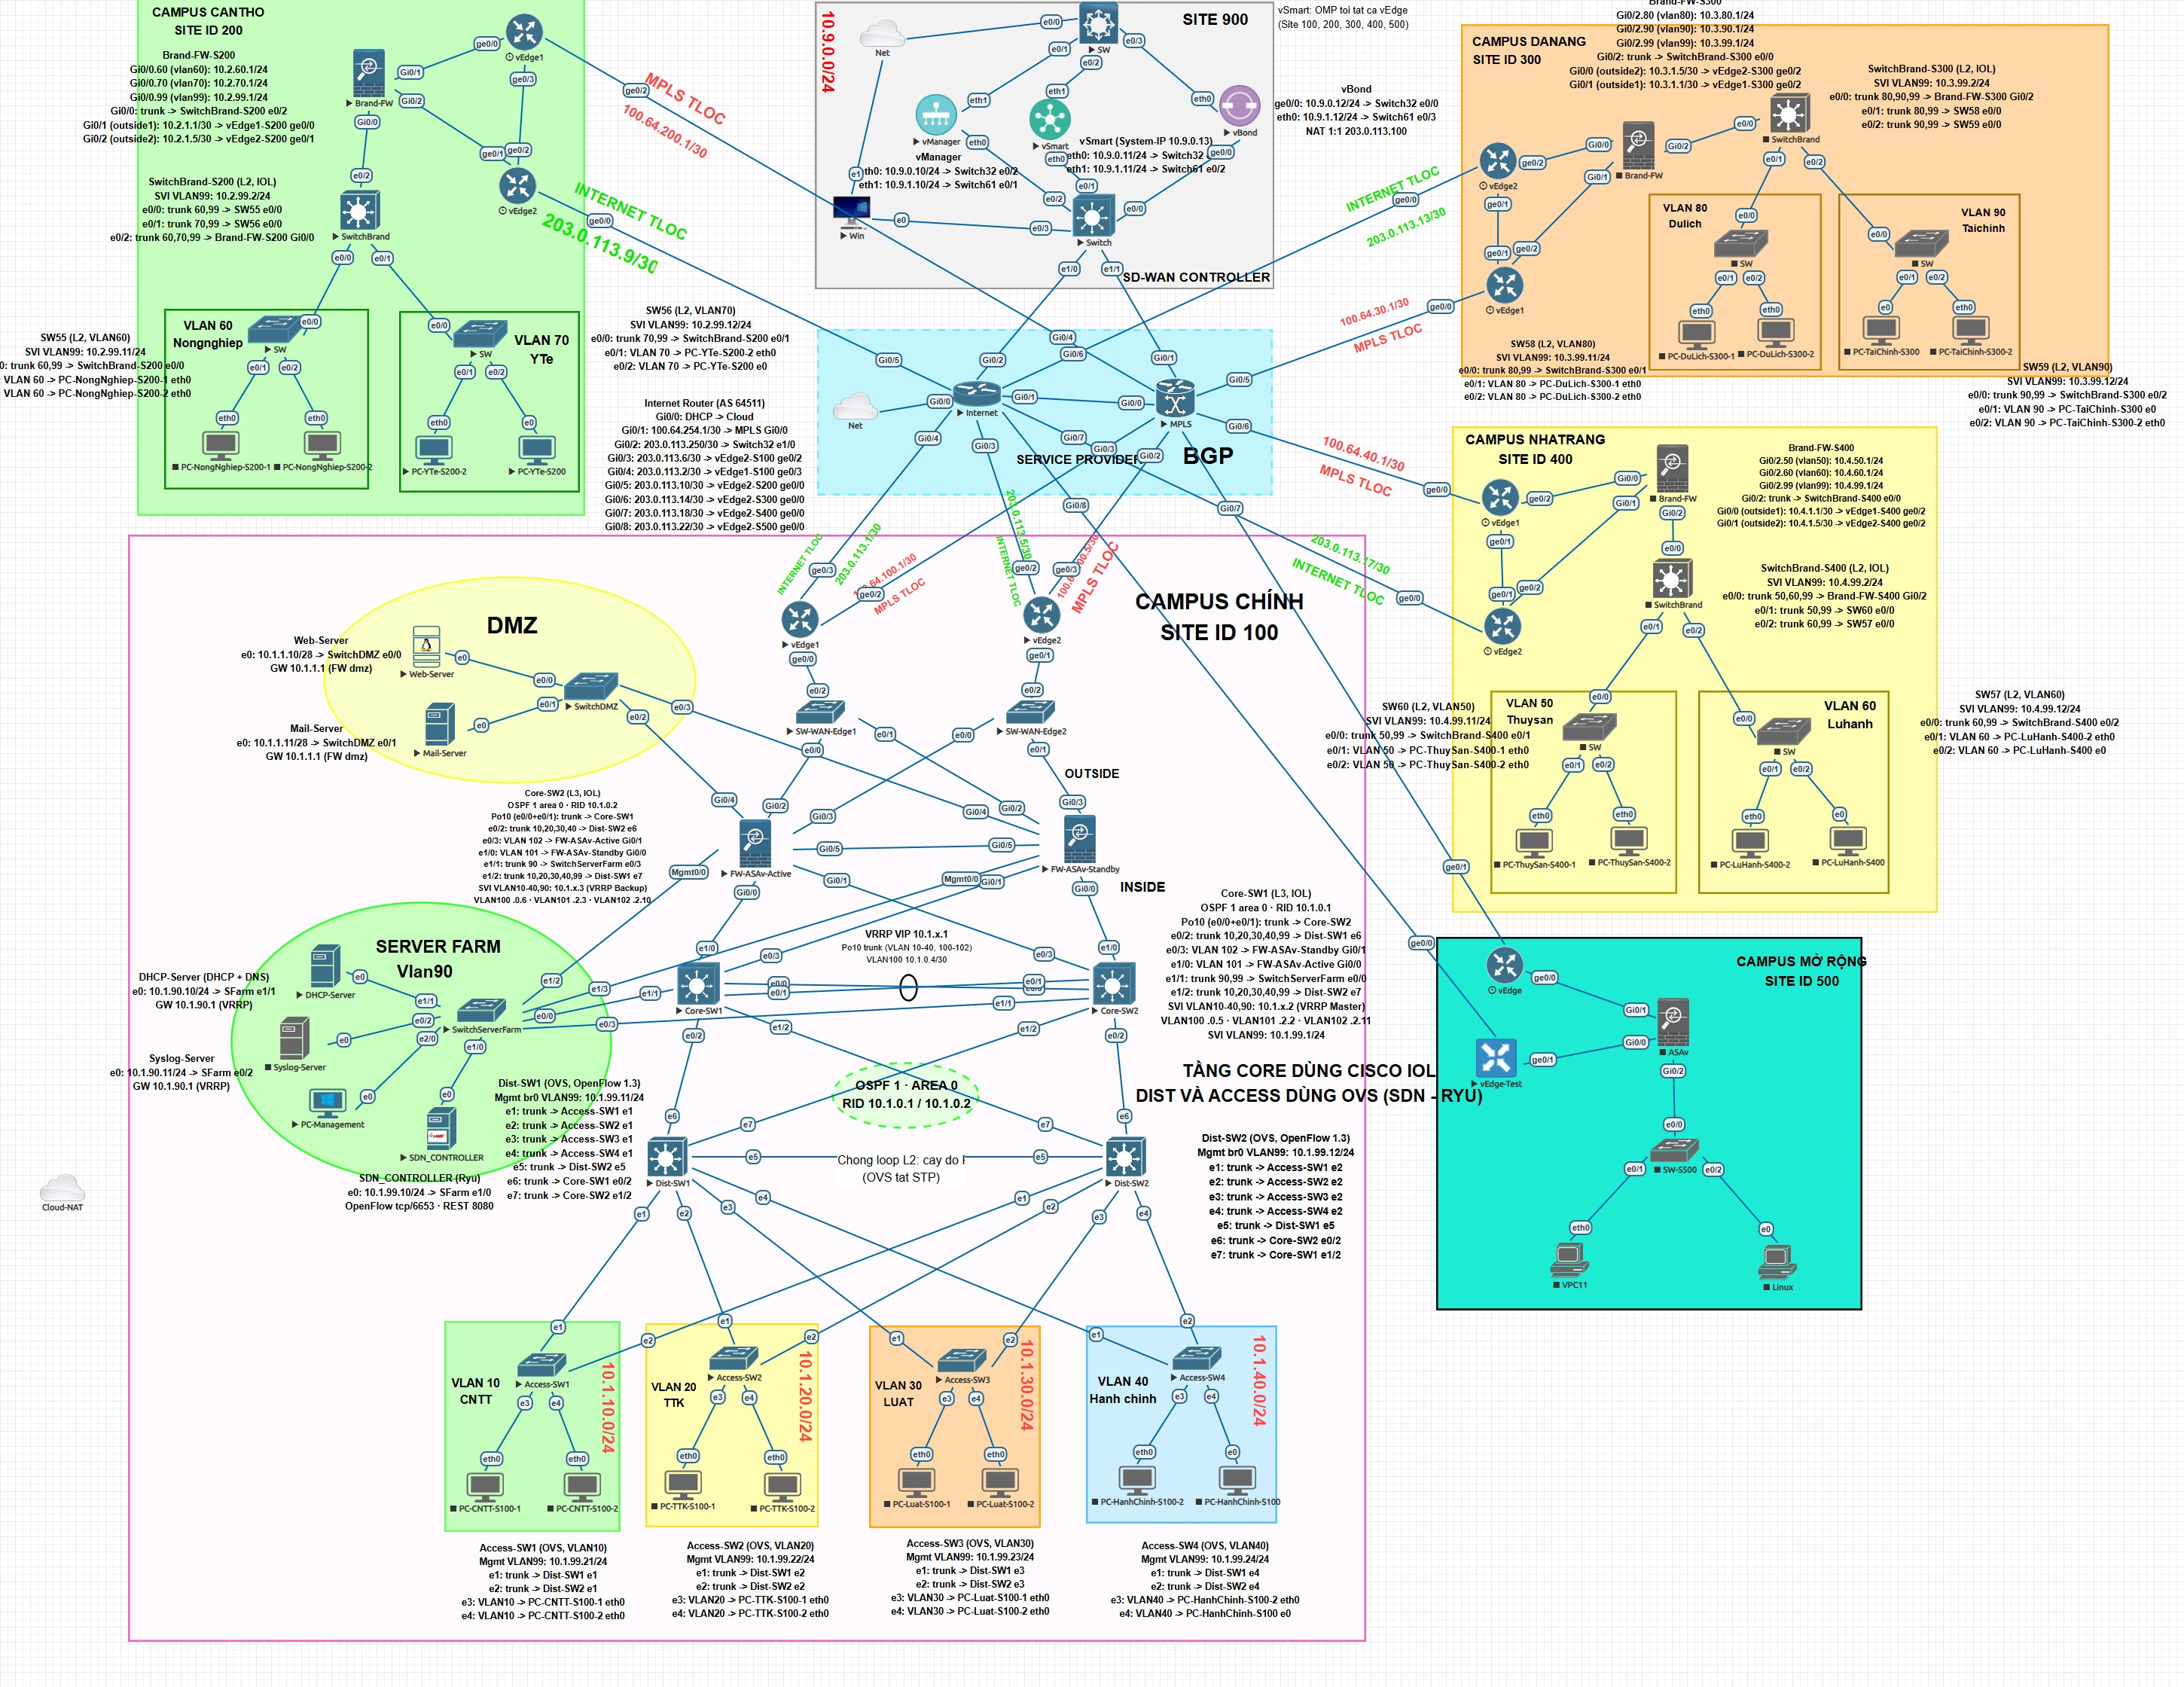
\includegraphics[height=0.985\paperheight]{topo_tongthe_0111.jpg}};
        \node[anchor=north west, text width=3.6cm, align=left, font=\scriptsize, text=ink]
            at ([xshift=0.55cm, yshift=-0.45cm]current page.north west)
            {{\tiny\color{inkSoft}MÔ HÌNH MẠNG CAMPUS ĐỀ XUẤT}\\[1pt]
             {\large\bfseries\color{navy}Topology vật lý}\\[2pt]
             \tikz\fill[brand] (0,0) rectangle (1.4cm,2pt);\tikz\fill[accent] (0,0) rectangle (0.5cm,2pt);\\[6pt]
             {\color{inkSoft}EVE-NG: 74 node, 107 phân đoạn mạng}\\[8pt]
             \textbf{\color{brand}Site 100} -- Campus chính: SDN (Ryu + 6 OVS), FW-ASAv HA qua SW-WAN-Edge1/2\\[4pt]
             \textbf{\color{brand}Site 200/300/400} -- cơ sở Cần Thơ, Đà Nẵng, Nha Trang\\[4pt]
             \textbf{\color{brand}Site 500} -- cơ sở mở rộng\\[4pt]
             \textbf{\color{brand}Site 900} -- SD-WAN controller\\[4pt]
             \textbf{\color{brand}Nhà cung cấp} -- Internet \& MPLS chạy BGP};
    \end{tikzpicture}
\end{frame}}

\begin{frame}{Campus chính (Site 100) -- ba tầng, tường lửa HA, SDN}
    \begin{columns}[c]
        \begin{column}{0.56\textwidth}
            \centering
            \begin{tikzpicture}[font=\tiny, y=0.88cm,
                dev/.style={draw, rounded corners=2pt, align=center, minimum height=0.52cm, text width=1.75cm, line width=0.6pt, inner sep=1.5pt},
                edge/.style={dev, draw=accent, fill=accentSoft},
                l2/.style={dev, draw=inkSoft, fill=paper},
                fw/.style={dev, draw=warnAmber, fill=warnSoft},
                core/.style={dev, draw=brand, fill=brandSoft},
                ovs/.style={dev, draw=okGreen, fill=okSoft},
                srv/.style={dev, draw=line, fill=white, text width=2.1cm},
                act/.style={line width=0.8pt, ink},
                stb/.style={dashed, line width=0.5pt, inkSoft}]
                \node[edge] (ve1) at (-3.1,6) {\textbf{vEdge1}\\Internet + MPLS};
                \node[edge] (ve2) at (3.1,6) {\textbf{vEdge2}\\Internet + MPLS};
                \node[l2] (w1) at (-3.1,5) {SW-WAN-Edge1};
                \node[l2] (w2) at (3.1,5) {SW-WAN-Edge2};
                \node[fw] (fa) at (-3.1,3.9) {\textbf{FW-ASAv Active}};
                \node[fw] (fs) at (3.1,3.9) {\textbf{FW-ASAv Standby}};
                \node[srv] (dmz) at (0,3.9) {\textbf{DMZ}: Web, Mail};
                \node[core] (c1) at (-3.1,2.7) {\textbf{Core-SW1}\\VRRP Master};
                \node[core] (c2) at (3.1,2.7) {\textbf{Core-SW2}\\VRRP Backup};
                \node[srv] (farm) at (0,2.7) {\textbf{Server Farm}\\DHCP/DNS, Syslog, Ryu};
                \node[ovs] (d1) at (-1.6,1.25) {\textbf{Dist-SW1} (OVS)};
                \node[ovs] (d2) at (1.6,1.25) {\textbf{Dist-SW2} (OVS)};
                \node[ovs, text width=1.45cm] (a1) at (-3.3,0) {Access-SW1\\VLAN 10};
                \node[ovs, text width=1.45cm] (a2) at (-1.1,0) {Access-SW2\\VLAN 20};
                \node[ovs, text width=1.45cm] (a3) at (1.1,0) {Access-SW3\\VLAN 30};
                \node[ovs, text width=1.45cm] (a4) at (3.3,0) {Access-SW4\\VLAN 40};
                \begin{scope}[on background layer]
                    \draw[act] (ve1) -- (w1) -- (fa); \draw[act] (ve2) -- (w2);
                    \draw[act] (w2) -- (fa.north east); \draw[stb] (w1) -- (fs.north west); \draw[stb] (w2) -- (fs);
                    \draw[act] (fa) -- (dmz); \draw[stb] (dmz) -- (fs);
                    \draw[act] (fa) -- (c1); \draw[act] (fa.south east) -- (c2.north west);
                    \draw[stb] (fs) -- (c2); \draw[stb] (fs.south west) -- (c1.north east);
                    \draw[brand, line width=1.2pt] ([yshift=1.6mm]c1.east) -- ([yshift=1.6mm]c2.west);
                    \draw[act] ([yshift=-1.4mm]c1.east) -- ([yshift=-1.4mm]c2.west);
                    \draw[warnAmber, line width=1.2pt] ([yshift=1.6mm]fa.east) -- ([yshift=1.6mm]fs.west);
                    \draw[act] (c1) -- (d1); \draw[act] (c1) -- (d2);
                    \draw[stb] (c2) -- (d1); \draw[stb] (c2) -- (d2); \draw[stb] (d1) -- (d2);
                    \foreach \a in {a1,a2,a3,a4} {\draw[act] (d1) -- (\a); \draw[stb] (d2) -- (\a);}
                \end{scope}
                \node[text=brand, fill=white, inner sep=0.8pt, anchor=south] at (1.68,2.9) {Po10};
                \node[text=warnAmber, fill=white, inner sep=0.8pt, anchor=south] at (1.68,4.1) {failover};
            \end{tikzpicture}
            \capt{Nét liền: đường đang dùng \,·\, nét đứt: dự phòng / cạnh bị Controller chặn}
        \end{column}
        \begin{column}{0.42\textwidth}
            \begin{card}{Phân vai rõ ràng}
                \scriptsize
                \begin{itemize}\compactlist
                    \item \textbf{Access/Distribution = OVS}, mỗi Access nối kép; chống vòng do Controller tính cây.
                    \item \textbf{Core IOL L3:} SVI + VRRP cho 5 VLAN, DHCP relay, OSPF; Po10 mang cả VLAN 10--40 để tránh VRRP split-brain.
                    \item \textbf{FW-ASAv Active/Standby:} transit dùng chung VLAN 101--104 (/29), OSPF với 2 Core và 2 vEdge.
                    \item \textbf{2 vEdge qua 2 SW-WAN-Edge:} không còn điểm lỗi đơn phía WAN.
                    \item \textbf{DMZ:} Web (Nginx), Mail (hMailServer).
                    \item \textbf{VLAN 99:} quản trị + kênh OpenFlow tới Ryu \texttt{10.1.99.10}.
                \end{itemize}
            \end{card}
        \end{column}
    \end{columns}
\end{frame}

\begin{frame}{Cơ sở phụ -- khuôn Firewall-as-Core, Site 500 và Site 900}
    \begin{columns}[c]
        \begin{column}{0.40\textwidth}
            \centering
            \begin{tikzpicture}[font=\tiny, y=0.95cm,
                dev/.style={draw, rounded corners=2pt, align=center, minimum height=0.55cm, text width=2.0cm, line width=0.6pt, inner sep=1.5pt},
                ln/.style={line width=0.8pt, ink}, lbl/.style={fill=white, inner sep=1pt, text=inkSoft}]
                \node[dev, draw=inkSoft, fill=paper] (mp) at (-1.5,5.3) {\textbf{MPLS} AS 64512};
                \node[dev, draw=inkSoft, fill=paper] (in) at (1.5,5.3) {\textbf{Internet} AS 64511};
                \node[dev, draw=accent, fill=accentSoft] (v1) at (-1.5,4.2) {\textbf{vEdge1}\\TLOC \texttt{mpls}};
                \node[dev, draw=accent, fill=accentSoft] (v2) at (1.5,4.2) {\textbf{vEdge2}\\TLOC \texttt{biz-internet}};
                \node[dev, draw=warnAmber, fill=warnSoft, text width=3.3cm] (fw) at (0,2.95) {\textbf{Brand-FW} (ASAv)\\gateway .1, DHCP, SLA/track chọn vEdge};
                \node[dev, draw=brand, fill=brandSoft] (sb) at (0,1.9) {\textbf{SwitchBrand} (L2)};
                \node[dev, draw=brand, fill=brandSoft, text width=1.7cm] (s1) at (-1.5,0.9) {Switch khối 1};
                \node[dev, draw=brand, fill=brandSoft, text width=1.7cm] (s2) at (1.5,0.9) {Switch khối 2};
                \node[dev, draw=line, text width=1.7cm] (p1) at (-1.5,0) {2 máy VLAN A};
                \node[dev, draw=line, text width=1.7cm] (p2) at (1.5,0) {2 máy VLAN B};
                \draw[ln] (mp) -- node[lbl]{eBGP} (v1); \draw[ln] (in) -- node[lbl]{eBGP} (v2);
                \draw[ln] (v1) -- (v2);
                \draw[ln] (v1) -- node[lbl, pos=0.4]{outside1} (fw); \draw[ln] (v2) -- node[lbl, pos=0.4]{outside2} (fw);
                \draw[ln] (fw) -- node[lbl]{trunk A, B, 99} (sb);
                \draw[ln] (sb) -- (s1); \draw[ln] (sb) -- (s2); \draw[ln] (s1) -- (p1); \draw[ln] (s2) -- (p2);
            \end{tikzpicture}
        \end{column}
        \begin{column}{0.58\textwidth}
            \begin{card}{Vì sao Firewall-as-Core?}
                \scriptsize
                \begin{itemize}\compactlist
                    \item Chi nhánh chỉ 2 VLAN $\Rightarrow$ \textbf{một thiết bị lớp 3 là đủ}.
                    \item Tường lửa vừa là gateway, vừa cấp DHCP, vừa kiểm soát overlay vào LAN $\Rightarrow$ ít hop, ít điểm lỗi.
                    \item vEdge đã là router WAN $\Rightarrow$ không cần thêm router chi nhánh.
                    \item Hai kiến trúc (3 tầng và Firewall-as-Core) \textbf{cùng tồn tại có chủ đích} theo quy mô.
                \end{itemize}
            \end{card}
            \begin{columns}[T]
                \begin{column}{0.49\linewidth}
                    \begin{card}[accent]{Site 500 -- mở rộng}
                        \scriptsize Dùng lại đúng khuôn: 2 vEdge, Brand-FW-S500, SW-S500, AS 65040; gateway \texttt{10.5.10.1}.
                    \end{card}
                \end{column}
                \begin{column}{0.49\linewidth}
                    \begin{card}[okGreen]{Site 900 -- controller}
                        \scriptsize LAN \texttt{10.9.0.0/24}, tới được từ cả 2 transport; ra Internet \textbf{có kiểm soát}.
                    \end{card}
                \end{column}
            \end{columns}
        \end{column}
    \end{columns}
\end{frame}

\begin{frame}{Quy hoạch VLAN và địa chỉ IP}
    \begin{columns}[T]
        \begin{column}{0.36\textwidth}
            \begin{card}{Quy tắc thống nhất \texttt{10.0.0.0/8}}
                \scriptsize
                \begin{itemize}\compactlist
                    \item Octet 2 = \textbf{mã site}: 1, 2, 3, 4, 5, 9.
                    \item Octet 3 = \textbf{VLAN ID}: \texttt{10.<site>.<VLAN>.0/24}.
                    \item \texttt{.1} gateway; \texttt{.10/.11} máy chủ; \texttt{.100--.199} DHCP.
                    \item Điểm--điểm \texttt{/30}; transit tường lửa \texttt{/29}.
                    \item Internet \texttt{203.0.113.0/24}; MPLS \texttt{100.64.x.x/30}.
                    \item System-IP \texttt{10.200.<site>.x}.
                \end{itemize}
            \end{card}
            \begin{softcard}\scriptsize
                Site mới chỉ cần cấp Site-ID, System-IP, subnet và ASN -- đã kiểm chứng với Site 500.
            \end{softcard}
        \end{column}
        \begin{column}{0.62\textwidth}
            \scriptsize
            \renewcommand{\arraystretch}{1.08}
            \rowcolors{2}{paper}{white}
            \begin{tabularx}{\linewidth}{@{}cL{0.34\linewidth}L{0.2\linewidth}Y@{}}
                \toprule
                \hd{VLAN} & \hd{Khu vực} & \hd{Subnet} & \hd{Gateway / ghi chú} \\
                \midrule
                10 & Khoa Công nghệ thông tin & 10.1.10.0/24 & VRRP .1, DHCP \\
                20 & Khoa Toán -- Thống kê & 10.1.20.0/24 & VRRP .1, DHCP \\
                30 & Khoa Luật & 10.1.30.0/24 & VRRP .1, DHCP \\
                40 & Khối Hành chính & 10.1.40.0/24 & VRRP .1, DHCP \\
                90 & Server Farm & 10.1.90.0/24 & DHCP/DNS .10, Syslog .11 \\
                99 & Quản trị, kênh SDN & 10.1.99.0/24 & Controller .10 \\
                101--104 & Transit FW -- Core -- vEdge & 10.1.2.x, 10.1.3.x /29 & OSPF Area 0 \\
                DMZ & Web, Mail & 10.1.1.0/28 & Web .10, Mail .11 \\
                \midrule
                60 / 70 & Site 200: Nông nghiệp / Y tế & 10.2.60/70.0/24 & Brand-FW .1 \\
                80 / 90 & Site 300: Du lịch / Tài chính & 10.3.80/90.0/24 & Brand-FW .1 \\
                50 / 60 & Site 400: Thủy sản / Lữ hành & 10.4.50/60.0/24 & Brand-FW .1 \\
                \bottomrule
            \end{tabularx}
        \end{column}
    \end{columns}
\end{frame}

\begin{frame}{Thiết kế định tuyến và luồng lưu lượng}
    \begin{columns}[T]
        \begin{column}{0.49\textwidth}
            \begin{card}{Ba miền định tuyến}
                \scriptsize
                \renewcommand{\arraystretch}{1.12}
                \begin{tabularx}{\linewidth}{@{}L{0.27\linewidth}Y@{}}
                    \hd{Campus chính} & \textbf{OSPF Area 0} giữa Core, tường lửa và vEdge; tường lửa phát default; vEdge đưa tuyến OMP vào OSPF (metric 10 / 100) \\
                    \hd{Underlay} & \textbf{eBGP} CE--PE với hai nhà cung cấp; Site 900 dùng tuyến tĩnh; lọc default chiều vào tại nhà cung cấp \\
                    \hd{Chi nhánh} & Brand-FW dùng \textbf{tuyến tĩnh + IP SLA/track}: nội bộ qua vEdge1 (MPLS), Internet qua vEdge2; tự đổi khi mất beacon \\
                    \hd{Overlay} & \textbf{OMP} phân phối tuyến VPN 1 giữa các site; control policy ưu tiên vEdge1 \\
                \end{tabularx}
            \end{card}
        \end{column}
        \begin{column}{0.49\textwidth}
            \begin{card}[accent]{Luồng lưu lượng}
                \scriptsize
                \begin{itemize}\compactlist
                    \item \textbf{Nội bộ Campus:} máy trạm $\rightarrow$ Access $\rightarrow$ Dist-SW1 (theo cây) $\rightarrow$ Core-SW1 (VRRP Master) $\rightarrow$ VLAN đích.
                    \item \textbf{Campus ra WAN:} Core $\rightarrow$ tường lửa Active $\rightarrow$ vEdge1 (chính) / vEdge2 (dự phòng) $\rightarrow$ IPsec theo AAR.
                    \item \textbf{Chi nhánh về Campus:} Brand-FW $\rightarrow$ vEdge1 $\rightarrow$ overlay $\rightarrow$ vEdge1-S100 $\rightarrow$ tường lửa biên (ACL \texttt{SDWAN\_IN}).
                    \item \textbf{Chi nhánh ra Internet:} DIA qua vEdge2, \textbf{không vòng qua Campus}; mất Internet thì ra qua MPLS.
                    \item \textbf{Chi nhánh $\leftrightarrow$ chi nhánh:} đường hầm trực tiếp (full-mesh).
                \end{itemize}
            \end{card}
        \end{column}
    \end{columns}
    \vspace{-0.05cm}
    \begin{softcard}\scriptsize
        \textbf{\color{brand}Nguyên tắc đối xứng:} control policy và tuyến mặc định đều chọn vEdge1 $\Rightarrow$ hai chiều đi qua cùng một cổng tường lửa trạng thái, không bị hủy gói.
    \end{softcard}
\end{frame}

\begin{frame}{Thiết kế SDN -- ứng dụng Ryu điều khiển lớp 2}
    \begin{columns}[T]
        \begin{column}{0.56\textwidth}
            \begin{card}{Ứng dụng \texttt{campus\_switch\_13.py} do nhóm xây dựng}
                \scriptsize
                \begin{enumerate}\compactlist
                    \item \textbf{Học MAC theo VLAN}; flood chỉ trong đúng VLAN, trên cây.
                    \item \textbf{Xử lý thẻ 802.1Q} theo OpenFlow 1.3 (\texttt{PUSH/POP\_VLAN}, \texttt{vlan\_vid}).
                    \item \textbf{Cây chuyển tiếp tính tập trung} (Dijkstra, gốc Core-SW1) trên đồ thị 13 liên kết; cạnh dư bị DROP.
                    \item \textbf{Thăm dò liên kết chủ động} 0,5\,s (OVS) và ARP 1\,s (Core) $\Rightarrow$ thấy cả lỗi ``đứt ngầm''.
                    \item \textbf{Phát RARP} thay máy trạm sau khi cây đổi để Core học lại MAC.
                    \item \textbf{VLAN động} và \textbf{chính sách tập trung} bằng một lệnh API.
                    \item \textbf{Northbound REST} cho Console và công cụ kiểm thử.
                \end{enumerate}
            \end{card}
        \end{column}
        \begin{column}{0.42\textwidth}
            \begin{card}[accent]{Hybrid SDN, kênh điều khiển in-band}
                \scriptsize
                \begin{itemize}\compactlist
                    \item Controller tại \texttt{10.1.99.10}, kênh OpenFlow đi trên \textbf{VLAN 99} của hạ tầng.
                    \item OVS: \texttt{OpenFlow13}, \texttt{fail\_mode=secure}, tắt STP, tắt in-band ẩn.
                    \item Core không chạy OpenFlow: giữ SVI, VRRP, OSPF.
                \end{itemize}
            \end{card}
            \begin{card}[okGreen]{Hai bảng flow}
                \scriptsize
                \textbf{Bảng 0 -- kiểm soát:} thăm dò, kênh quản trị, chặn cạnh ngoài cây, chính sách.\\
                \textbf{Bảng 1 -- chuyển tiếp:} unicast đã học; table-miss $\rightarrow$ Controller.
            \end{card}
        \end{column}
    \end{columns}
\end{frame}

\begin{frame}{Thiết kế SDN -- cây dữ liệu, kênh VLAN 99 và tự phục hồi}
    \begin{columns}[T]
        \begin{column}{0.50\textwidth}
            \centering
            \shot{sdn-console-topology.png}
            \capt{Cây dữ liệu khi bình thường: gốc Core-SW1, bốn Access đi lên Dist-SW1 (xanh: thuộc cây, xám: dự phòng)}
            \vspace{0.1cm}
            \begin{softcard}[okSoft]\scriptsize
                \textbf{\color{okGreen}Tự phục hồi an toàn:} mất kênh điều khiển $\neq$ liên kết chết \,·\,
                Access mất kết nối được ``đóng băng'' trên liên kết cũ \,·\, có ân hạn khi Controller khựng.
            \end{softcard}
        \end{column}
        \begin{column}{0.48\textwidth}
            \begin{card}{Kênh quản trị VLAN 99 không phụ thuộc STP}
                \scriptsize
                \begin{itemize}\compactlist
                    \item \textbf{Không vòng qua Core:} khung vào từ cổng Core không bao giờ ra cổng Core khác.
                    \item \textbf{Nhiều đường đồng thời:} mỗi Access có 4 đường, mỗi Distribution có 2 đường tới Controller $\Rightarrow$ không cần chuyển mạch khi sự cố.
                    \item \textbf{Chống phản xạ} theo MAC nguồn của sáu OVS.
                \end{itemize}
            \end{card}
            \begin{card}[accent]{Giải vòng phụ thuộc khi khởi động}
                \scriptsize
                Switch cần flow để tới Controller, Controller lại chỉ tới được qua switch $\Rightarrow$ mỗi OVS có \textbf{dịch vụ khởi động} cài flow bootstrap cho VLAN 99; flow quản trị luôn \textbf{ghi đè}, không xóa trước.
            \end{card}
        \end{column}
    \end{columns}
\end{frame}

\begin{frame}{Thiết kế SD-WAN -- overlay và chính sách tập trung}
    \begin{columns}[T]
        \begin{column}{0.40\textwidth}
            \begin{card}{Overlay full-mesh}
                \scriptsize
                \begin{itemize}\compactlist
                    \item \textbf{PKI:} Root CA riêng, mỗi Edge có chứng thư và nằm trong danh sách hợp lệ của 3 controller.
                    \item \textbf{VPN 0} transport + BGP; \textbf{VPN 1} dịch vụ; \textbf{VPN 512} quản trị.
                    \item 10 Edge, \textbf{12 TLOC}: Edge Site 100 có 16 phiên BFD, Edge chi nhánh có 10.
                    \item App-route tổng hợp mỗi 120\,s để AAR phản ứng nhanh hơn.
                \end{itemize}
            \end{card}
            \begin{softcard}\scriptsize
                \textbf{SLA\_REALTIME:} mất $\le$2\,\%, trễ $\le$150\,ms, jitter $\le$50\,ms\\
                \textbf{SLA\_BUSINESS:} mất $\le$5\,\%, trễ $\le$300\,ms, jitter $\le$100\,ms
            \end{softcard}
        \end{column}
        \begin{column}{0.58\textwidth}
            \begin{card}[accent]{Chính sách khai một lần trên vSmart, áp theo danh sách site}
                \scriptsize
                \renewcommand{\arraystretch}{1.12}
                \begin{tabularx}{\linewidth}{@{}L{0.25\linewidth}Y@{}}
                    \hd{AAR\_LAN} & Phân loại theo ứng dụng, chọn đường hầm thỏa SLA: ICMP và thoại (DSCP 46) $\rightarrow$ REALTIME; Server Farm, Web, Mail $\rightarrow$ BUSINESS; mỗi lớp có bộ đếm \\
                    \hd{DP\_BRANCH} & Data policy cho mọi chi nhánh: chặn Telnet vào Server Farm, chặn SSH/Telnet vào DMZ, đếm ICMP \\
                    \hd{PREFER-VE1} & Control policy: tuyến của vEdge1 mỗi site có preference 200 $\Rightarrow$ lưu lượng đối xứng qua tường lửa \\
                    \hd{Cảnh báo} & vManage gửi email khi BFD/Control/OMP Down và khi phục hồi \\
                \end{tabularx}
            \end{card}
            \begin{softcard}[okSoft]\scriptsize
                Danh sách site khai theo dải (100--500) $\Rightarrow$ cơ sở mới \textbf{tự nhận chính sách} khi vào fabric.
            \end{softcard}
        \end{column}
    \end{columns}
\end{frame}

\begin{frame}{Thiết kế dịch vụ, Internet và bảo mật nhiều lớp}
    \begin{columns}[T]
        \begin{column}{0.33\textwidth}
            \begin{card}{Dịch vụ dùng chung}
                \scriptsize
                \renewcommand{\arraystretch}{1.08}
                \begin{tabularx}{\linewidth}{@{}L{0.26\linewidth}Y@{}}
                    DHCP & Windows Server, 4 scope qua relay; chi nhánh do Brand-FW cấp \\
                    DNS & Zone \texttt{campus.internal}, chuyển tiếp tên ngoài \\
                    Web & Nginx HTTPS trong DMZ \\
                    Mail & hMailServer: SMTP 587, IMAP \\
                    Syslog & Kiwi Syslog, UDP 514 \\
                \end{tabularx}
            \end{card}
        \end{column}
        \begin{column}{0.32\textwidth}
            \begin{card}[accent]{Internet tại chỗ (DIA)}
                \scriptsize
                \begin{itemize}\compactlist
                    \item \textbf{NAT hai tầng:} vEdge NAT, nhà cung cấp PAT ra mạng thật.
                    \item \textbf{Dự phòng qua MPLS} khi đường Internet của site hỏng.
                    \item \textbf{Split DNS:} chỉ máy chủ DNS được hỏi ra ngoài.
                    \item \textbf{Giới hạn theo vùng:} VLAN 99 không ra Internet; Server Farm, DMZ, Site 900 chỉ dịch vụ cần thiết.
                \end{itemize}
            \end{card}
        \end{column}
        \begin{column}{0.33\textwidth}
            \begin{card}[okGreen]{Bảo mật nhiều lớp}
                \scriptsize
                \begin{itemize}\compactlist
                    \item \textbf{Tường lửa biên:} 3 ACL theo hướng \texttt{SDWAN\_IN}, \texttt{DMZ\_IN}, \texttt{INSIDE\_OUT}.
                    \item \textbf{Overlay:} data policy chặn truy cập quản trị từ chi nhánh.
                    \item \textbf{SDN:} luật theo VLAN, địa chỉ, cổng tại Access.
                    \item \textbf{Điều khiển:} DTLS/IPsec, chứng thư; OpenFlow trong VLAN 99; ASDM chỉ từ mạng quản trị.
                \end{itemize}
            \end{card}
        \end{column}
    \end{columns}
    \vspace{-0.05cm}
    \begin{softcard}\scriptsize
        Một luồng từ chi nhánh vào DMZ phải thỏa \textbf{đồng thời} chính sách overlay và ACL tường lửa biên -- hai lớp kiểm soát độc lập.
    \end{softcard}
\end{frame}

% ============================================================
% 04. TRIỂN KHAI VÀ KIỂM THỬ
% ============================================================
\section{Triển khai và kiểm thử}

\begin{frame}{Môi trường triển khai và phương pháp kiểm thử}
    \begin{columns}[T]
        \begin{column}{0.60\textwidth}
            \scriptsize
            \renewcommand{\arraystretch}{1.08}
            \rowcolors{2}{paper}{white}
            \begin{tabularx}{\linewidth}{@{}L{0.25\linewidth}L{0.33\linewidth}cY@{}}
                \toprule
                \hd{Nhóm} & \hd{Nền tảng} & \hd{SL} & \hd{Thiết bị} \\
                \midrule
                Tường lửa & Cisco ASAv 9.20 & 6 & FW HA Site 100, 4 Brand-FW \\
                Switch Cisco & Cisco IOL L2/L3 & 18 & Core, DMZ, Server Farm, chi nhánh \\
                Nhà cung cấp & Cisco vIOS 15.7 & 2 & Internet, MPLS \\
                SD-WAN Controller & Viptela 20.10.1 & 3 & vManage, vSmart, vBond \\
                SD-WAN Edge & vEdge Cloud 20.10.1 & 10 & 2 vEdge mỗi site 100--500 \\
                SDN & Ubuntu + OVS; Ryu & 7 & 6 OVS, 1 Controller \\
                Máy chủ, máy trạm & Ubuntu, Windows & 11 & Web, DHCP/DNS, Mail, Syslog, PC \\
                Máy trạm giả lập & VPCS & 17 & Site 100--500 \\
                \bottomrule
            \end{tabularx}
        \end{column}
        \begin{column}{0.38\textwidth}
            \begin{card}{Nguyên tắc}
                \scriptsize
                \begin{itemize}\compactlist
                    \item Thiết kế, topology và cấu hình \textbf{thống nhất}, quản lý bằng Git.
                    \item \textbf{Từ dưới lên:} underlay trước overlay, kết nối trước chính sách.
                    \item \textbf{Chẩn đoán theo lớp}, dừng ở lớp đầu tiên sai, có bằng chứng.
                    \item Phép đo lặp lại bằng \textbf{script}; cắt liên kết \textbf{thật} trên máy chủ.
                \end{itemize}
            \end{card}
            \begin{softcard}\scriptsize
                Ba mức kết quả: \textbf{Đạt} \,·\, Đạt một phần \,·\, Chưa nghiệm thu.
            \end{softcard}
        \end{column}
    \end{columns}
\end{frame}

\begin{frame}{Campus chính -- VRRP, OSPF và tường lửa HA}
    \begin{columns}[T]
        \begin{column}{0.40\textwidth}
            \begin{card}{Trạng thái thực tế}
                \scriptsize
                \begin{itemize}\compactlist
                    \item Core-SW1 \textbf{Master}, Core-SW2 \textbf{Backup} ở cả 5 VLAN; Po10 đủ 2/2 cổng.
                    \item FW: \textbf{Active} / \textbf{Standby Ready}, \texttt{Sync Done}.
                    \item Tường lửa có \textbf{6 láng giềng OSPF FULL}; ASDM từ VLAN 99.
                \end{itemize}
            \end{card}
            \begin{card}[accent]{Ba lỗi đã xử lý}
                \scriptsize
                \begin{itemize}\compactlist
                    \item Standby ở mạng /30 khác, failover chưa từng chạy $\Rightarrow$ transit chung /29.
                    \item VRRP \textbf{split-brain} $\Rightarrow$ đưa VLAN 10--40 lên Po10.
                    \item ASAv khởi động lại lặp do \texttt{track} $\Rightarrow$ đổi đích thăm dò.
                \end{itemize}
            \end{card}
        \end{column}
        \begin{column}{0.58\textwidth}
            \centering
            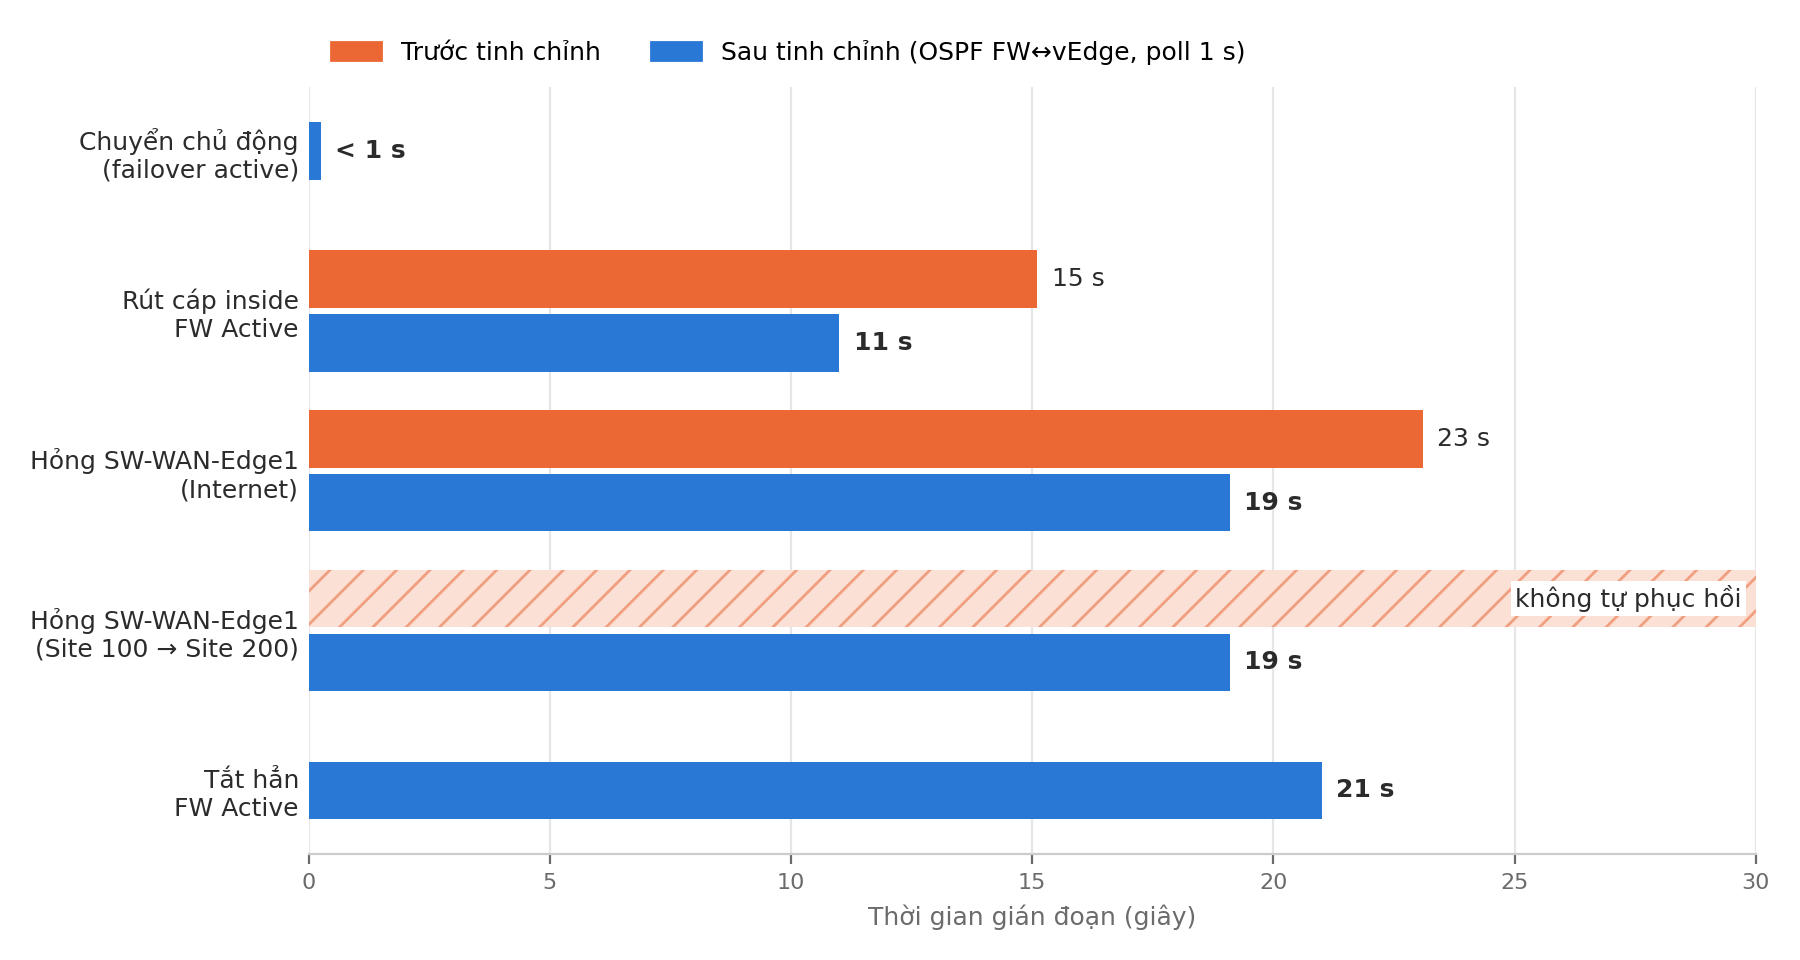
\includegraphics[width=\linewidth]{fw_ha_failover.png}
            \capt{Thời gian gián đoạn khi gây lỗi cặp tường lửa HA, trước và sau tinh chỉnh}
            \vspace{0.05cm}
            \begin{softcard}[okSoft]\scriptsize
                Chuyển chủ động \textbf{dưới 1\,s} \,·\, rút cáp inside \textbf{11\,s} \,·\, hỏng SW-WAN-Edge1 \textbf{19\,s} \,·\, tắt hẳn Active \textbf{21\,s}.
            \end{softcard}
        \end{column}
    \end{columns}
\end{frame}

\begin{frame}{Campus SDN Console -- giám sát tập trung do nhóm phát triển}
    \begin{columns}[c]
        \begin{column}{0.62\textwidth}
            \centering
            \shot{sdn-console-tongquan.png}
            \capt{Trang Tổng quan: 6/6 switch, 13/13 liên kết, thời gian hội tụ và nhật ký sự kiện}
        \end{column}
        \begin{column}{0.36\textwidth}
            \begin{card}{Mười trang chức năng}
                \scriptsize
                \begin{itemize}\compactlist
                    \item \textbf{Tổng quan}, \textbf{Topology} (cắt/khôi phục liên kết).
                    \item \textbf{Khôi phục}: ping liên tục, thời gian phát hiện và hội tụ.
                    \item \textbf{Lưu lượng}, \textbf{Tải thiết bị}, \textbf{Hiệu năng}.
                    \item \textbf{VLAN}, \textbf{Chính sách} có bộ đếm.
                    \item \textbf{Sức khỏe} kênh điều khiển.
                    \item \textbf{Kịch bản} tự động S1--S6.
                \end{itemize}
            \end{card}
            \begin{softcard}\scriptsize
                Chạy ngay trong tiến trình Ryu, không dùng thư viện ngoài; mọi thao tác đều gọi REST API $\Rightarrow$ tự động hóa được.
            \end{softcard}
        \end{column}
    \end{columns}
\end{frame}

\begin{frame}{SDN -- thêm VLAN và áp chính sách bằng một lệnh}
    \begin{columns}[T]
        \begin{column}{0.49\textwidth}
            \centering
            \shot{sdn-console-vlan-20261108.png}
            \capt{Trang VLAN: năm VLAN và cổng access trên các OVS}
        \end{column}
        \begin{column}{0.49\textwidth}
            \centering
            \shot{sdn-console-chinhsach-20261108.png}
            \capt{Trang Chính sách: luật chặn ICMP VLAN 10 -- VLAN 40 khớp 5 gói}
            \vspace{0.1cm}
            \begin{softcard}\scriptsize
                Luật cài lên 4 Access (12 flow-mod): 5/5 gói bị chặn, bộ đếm tăng đúng 5; VLAN 20 vẫn thông.
            \end{softcard}
        \end{column}
    \end{columns}
    \vspace{-0.1cm}
    \begin{columns}[T]
        \begin{column}{0.235\textwidth}\stat{brand}{3,8 ms}{thêm VLAN trên 6 OVS (1 lệnh API)}\end{column}
        \begin{column}{0.235\textwidth}\stat{accent}{5,3 s}{xong SDN + hai Core; máy trạm dùng được sau $\approx$40\,s}\end{column}
        \begin{column}{0.235\textwidth}\stat{okGreen}{8--12,6 ms}{áp chính sách toàn campus}\end{column}
        \begin{column}{0.235\textwidth}\stat{brand}{18 lệnh}{CLI trên mỗi Core nếu làm truyền thống}\end{column}
    \end{columns}
\end{frame}

\begin{frame}{SDN -- kết quả theo năm tiêu chí định lượng}
    \vspace{0.05cm}
    \scriptsize
    \renewcommand{\arraystretch}{1.22}
    \rowcolors{2}{paper}{white}
    \begin{tabularx}{\textwidth}{@{}L{0.21\textwidth}Yc@{}}
        \toprule
        \hd{Tiêu chí} & \hd{Kết quả đo} & \hd{Đánh giá} \\
        \midrule
        Thời gian thêm VLAN & SDN \textbf{3,8\,ms}; xong SDN và hai Core sau \textbf{5,3\,s}; ping gateway sau 37,8\,s, DHCP Server sau 42,0\,s (3 lần đo) & \pass \\
        Thời gian khôi phục khi mất liên kết & Controller hội tụ \textbf{dưới 16\,ms}; gián đoạn chủ yếu là thời gian phát hiện: cổng down 0--0,3\,s, đứt ngầm Access--Distribution 1,8\,s, Distribution--Core 2,9--3,4\,s & \pass \\
        Hiệu năng giữa các VLAN & RTT \textbf{0,43\,ms} cùng VLAN, \textbf{1,57\,ms} khác VLAN, jitter dưới 0,4\,ms, mất gói \textbf{0\,\%} (490/490) khi 69/74 node chạy; TCP 1,2\,Gbit/s cùng Access, 170\,Mbit/s liên VLAN & \pass \\
        Tải Core / Distribution & Rảnh $\approx$85 packet-in/s, Ryu $\approx$4\,\% CPU, không tăng theo lưu lượng người dùng; 1000 MAC mới/giây $\Rightarrow$ Ryu 41,3\,\% CPU, luồng đang chạy không mất gói & \pass \\
        Áp chính sách tập trung & Áp \textbf{8,0--12,6\,ms}, gỡ 5,2--10,8\,ms trên bốn Access; bộ đếm khớp 5/5; luồng khác không ảnh hưởng & \pass \\
        \bottomrule
    \end{tabularx}
    \vspace{0.1cm}
    \begin{softcard}\scriptsize
        \textbf{\color{brand}Chức năng cơ bản:} 6/6 switch OpenFlow 1.3, 13/13 liên kết; 8 máy trạm nhận DHCP đủ DORA, thông liên VLAN;
        khởi động lại Controller: sáu switch nối lại sau $\approx$15\,s; không còn bão broadcast (365 gói/s so với 200.000 gói/s trước khắc phục).
    \end{softcard}
\end{frame}

\begin{frame}{SDN -- sáu kịch bản tự phục hồi S1--S6}
    \begin{columns}[c]
        \begin{column}{0.55\textwidth}
            \centering
            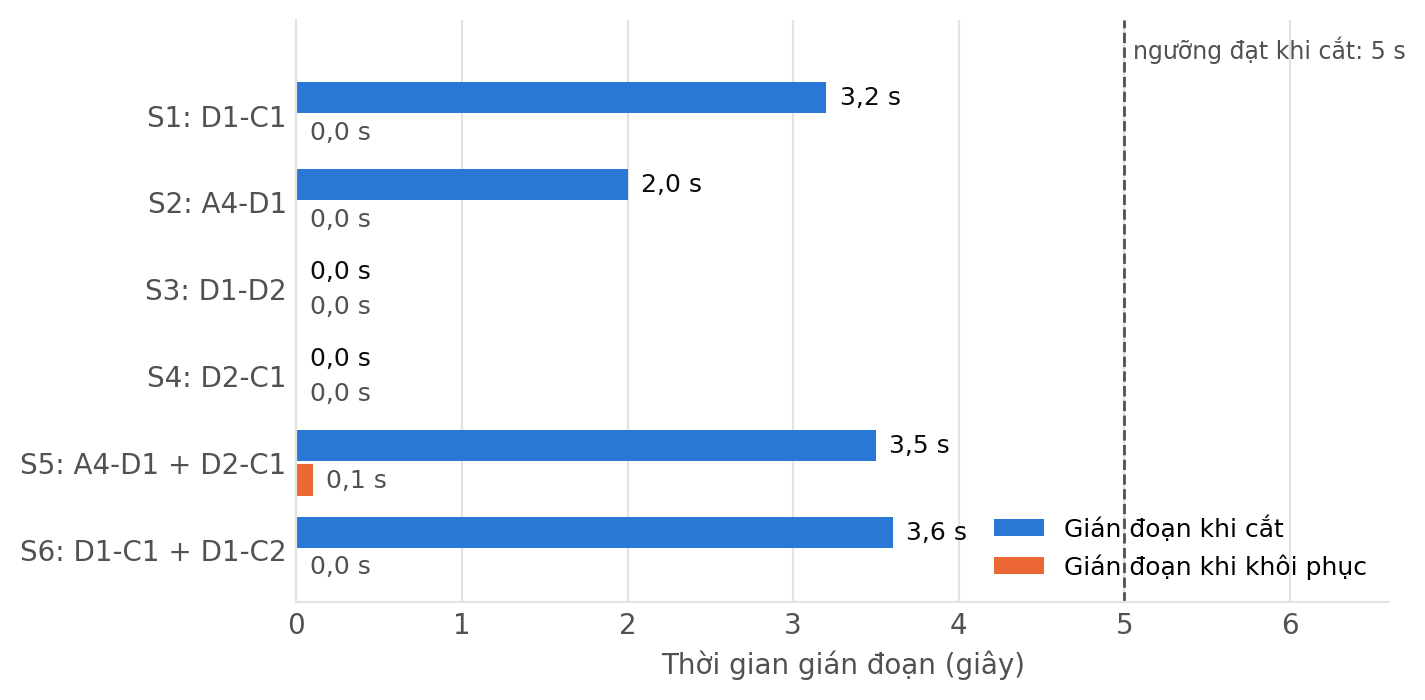
\includegraphics[width=\linewidth]{bd-sdn-kichban.png}
            \capt{Gián đoạn của sáu kịch bản so với ngưỡng đạt 5 giây}
        \end{column}
        \begin{column}{0.43\textwidth}
            \centering
            \shot{sdn-console-kichban-20261108.png}
            \capt{Trang Kịch bản: S1--S6 đều Đạt}
        \end{column}
    \end{columns}
    \vspace{0.05cm}
    \begin{columns}[T]
        \begin{column}{0.49\textwidth}
            \begin{softcard}[okSoft]\scriptsize
                \textbf{\color{okGreen}6/6 kịch bản đạt:} gián đoạn khi cắt \textbf{không quá 3,6\,s}, khi khôi phục không quá 0,1\,s;
                mạng về đủ 13/13 liên kết sau 1,5--2,5\,s; không switch nào mất Controller.
            \end{softcard}
        \end{column}
        \begin{column}{0.49\textwidth}
            \begin{softcard}\scriptsize
                \textbf{Cắt thật} (hạ giao diện trên máy chủ) cho kết quả tương tự; tắt hẳn Dist-SW2 chỉ mất 0--5 gói.
                Trước khi thiết kế lại kênh VLAN 99: S4, S5 \textbf{không đạt} (tới 15\,s).
            \end{softcard}
        \end{column}
    \end{columns}
\end{frame}

\begin{frame}{SDN -- đo dưới tải cao}
    \begin{columns}[T]
        \begin{column}{0.57\textwidth}
            \scriptsize
            \renewcommand{\arraystretch}{1.12}
            \rowcolors{2}{paper}{white}
            \begin{tabularx}{\linewidth}{@{}L{0.33\linewidth}L{0.2\linewidth}Y@{}}
                \toprule
                \hd{Đường đo (iperf3)} & \hd{TCP (Mbit/s)} & \hd{UDP: mất gói (tốc độ phát)} \\
                \midrule
                Cùng VLAN, cùng Access & 1184--1265 & 0\,\% (tới 500\,Mbit/s) \\
                Liên VLAN qua Core & 165--173 & $\le$0,07\,\% (tới 100\,Mbit/s) \\
                VLAN 10 tới Server Farm & 180--220 & $\le$0,05\,\% (tới 50\,Mbit/s) \\
                Qua ASAv (DMZ, liên site) & $\approx$0,08--0,09 & ASAv không giấy phép \\
                \bottomrule
            \end{tabularx}
            \vspace{0.1cm}
            \begin{card}{Ba nhận xét}
                \scriptsize
                \begin{itemize}\compactlist
                    \item \textbf{Dữ liệu không ảnh hưởng mặt phẳng điều khiển:} 64 phép đo, ping Controller 6321/6321, luôn 6/6 switch.
                    \item Liên VLAN giới hạn $\approx$170\,Mbit/s, nhiều khả năng do Core IOL chuyển mạch bằng phần mềm.
                    \item $\approx$0,1\,Mbit/s qua tường lửa là \textbf{giới hạn môi trường}, không phải của thiết kế.
                \end{itemize}
            \end{card}
        \end{column}
        \begin{column}{0.41\textwidth}
            \centering
            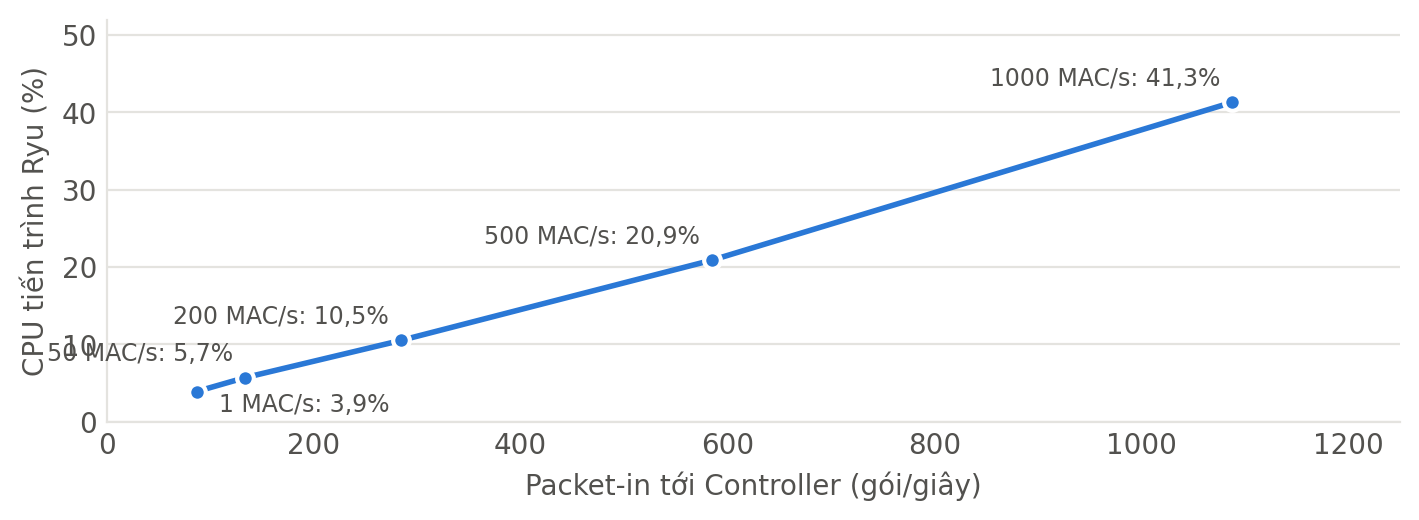
\includegraphics[width=\linewidth]{bd-sdn-packetin.png}
            \capt{CPU của Ryu theo tải packet-in}
            \vspace{0.1cm}
            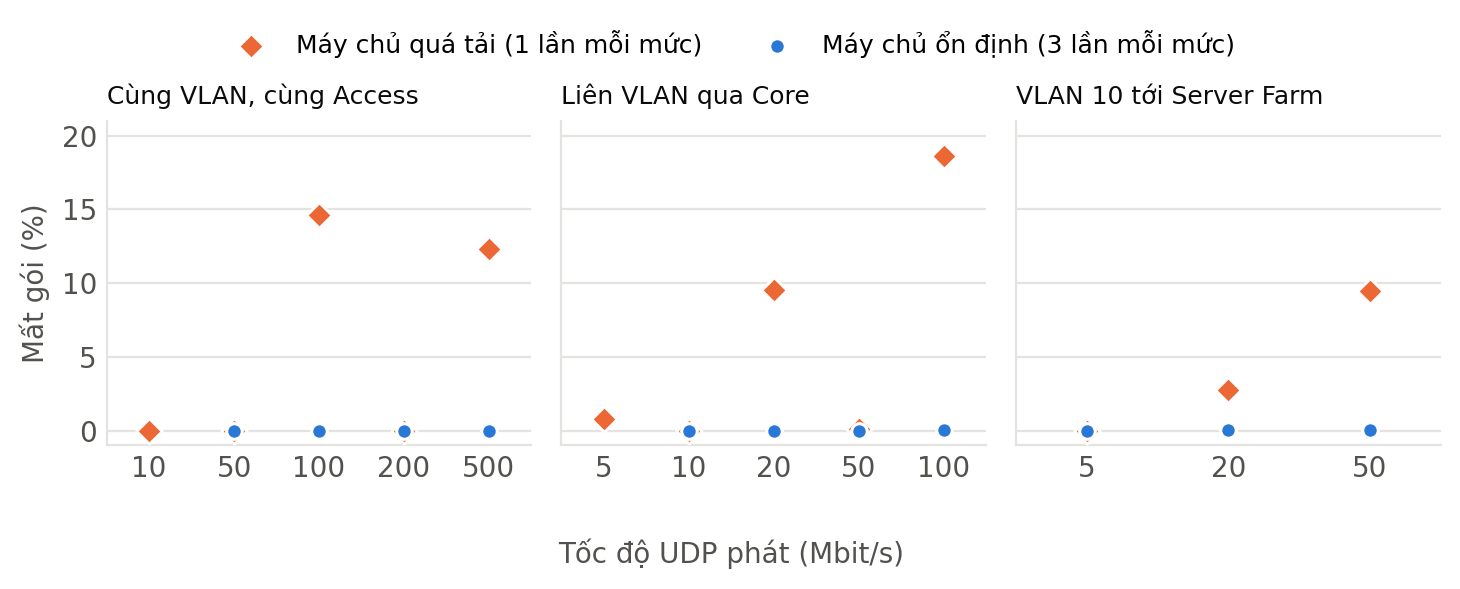
\includegraphics[width=\linewidth]{bd-sdn-udp-haitrangthai.png}
            \capt{Mất gói UDP ở hai trạng thái máy chủ: mất gói đến từ máy chủ quá tải, không phải từ SDN}
        \end{column}
    \end{columns}
\end{frame}

\begin{frame}{SDN -- vấn đề kỹ thuật và nguyên nhân gốc}
    \vspace{0.05cm}
    \scriptsize
    \renewcommand{\arraystretch}{1.2}
    \rowcolors{2}{paper}{white}
    \begin{tabularx}{\textwidth}{@{}L{0.25\textwidth}L{0.36\textwidth}Y@{}}
        \toprule
        \hd{Hiện tượng} & \hd{Nguyên nhân gốc} & \hd{Khắc phục} \\
        \midrule
        DHCP chỉ có Discover/Offer, thiếu Request/ACK & Flow dùng trường \texttt{dl\_vlan} của OpenFlow 1.0, gây ngoại lệ & Dùng \texttt{vlan\_vid} theo OpenFlow 1.3 \\
        Bão ARP $\approx$200.000 gói/s mỗi khi một OVS khởi động lại & Chế độ in-band của OVS tự cài flow \textbf{ẩn} hành động \texttt{NORMAL} & Tắt in-band (\texttt{disable-in-band=true}) \\
        Sau khi cây đổi, dữ liệu vẫn mất thêm 11--12\,s & Core (switch truyền thống) giữ vị trí MAC cũ & Controller phát RARP thay máy trạm \\
        Khôi phục liên kết D2--C1 làm 6 OVS mất Controller tới 10\,s & Core nghe chính BPDU của mình qua khối OVS $\Rightarrow$ RSTP \textit{Dispute} & Thiết kế lại kênh VLAN 99 không phụ thuộc STP \\
        Controller khựng 0,5--9\,s theo cụm & ONOS chạy song song chiếm hơn một vCPU & Tắt ONOS, ưu tiên CPU cho Ryu, thêm ân hạn \\
        Tắt Dist-SW2 làm 4 VLAN mất 100\,\% $\approx$3,5 phút & Controller chặn cổng xuống các Access mất kết nối & ``Đóng băng'' Access làm lá trên liên kết cũ \\
        \bottomrule
    \end{tabularx}
    \vspace{0.08cm}
    \begin{softcard}[accentSoft]\scriptsize
        \textbf{\color{accent}Bài học:} trong SDN in-band, mặt phẳng điều khiển phải được thiết kế như một mạng riêng (không vòng, nhiều đường, khởi động độc lập với Controller)
        trước khi xây logic cho mặt phẳng dữ liệu; mọi kết luận dựa trên bắt gói, trạng thái STP, thống kê CPU.
    \end{softcard}
\end{frame}

\begin{frame}{SD-WAN -- trạng thái fabric trên vManage}
    \begin{columns}[T]
        \begin{column}{0.49\textwidth}
            \centering
            \shot{vmanage-overview-20261107.png}
            \capt{Trang tổng quan: 3 controller, 10 WAN Edge reachable, 5 site, 112 đường hầm ở mức tốt}
            \vspace{0.1cm}
            \begin{softcard}\scriptsize
                \textbf{\color{brand}Đưa vEdge vào fabric:} cấu hình cơ sở $\rightarrow$ tuyến tới controller $\rightarrow$ tạo CSR, ký bằng Root CA
                $\rightarrow$ cài chứng thư $\rightarrow$ đăng ký chassis/serial trên cả 3 controller.
            \end{softcard}
        \end{column}
        \begin{column}{0.49\textwidth}
            \centering
            \shot{vmanage-devices-20261107.png}
            \capt{Danh sách thiết bị: kết nối điều khiển và số phiên BFD của từng vEdge}
        \end{column}
    \end{columns}
    \vspace{-0.05cm}
    \begin{columns}[T]
        \begin{column}{0.235\textwidth}\stat{brand}{10/10}{vEdge reachable, đã xác thực PKI}\end{column}
        \begin{column}{0.235\textwidth}\stat{okGreen}{3/3}{controller vManage, vSmart, vBond}\end{column}
        \begin{column}{0.235\textwidth}\stat{accent}{112}{đường hầm; BFD 16/16 (Site 100), 10/10 (chi nhánh)}\end{column}
        \begin{column}{0.235\textwidth}\stat{brand}{MOS $\approx$4,4}{ước lượng E-model; 0\,\% mất, 37\,ms, jitter 6\,ms}\end{column}
    \end{columns}
\end{frame}

\begin{frame}{SD-WAN -- kiểm chứng chính sách tập trung bằng bộ đếm}
    \begin{columns}[T]
        \begin{column}{0.62\textwidth}
            \scriptsize
            \renewcommand{\arraystretch}{1.12}
            \rowcolors{2}{paper}{white}
            \begin{tabularx}{\linewidth}{@{}cL{0.40\linewidth}Yc@{}}
                \toprule
                \hd{Mã} & \hd{Phép thử} & \hd{Thay đổi quan sát} & \\
                \midrule
                W-1 & vBond đủ danh sách vEdge hợp lệ & Không thiếu serial & \pass \\
                DP-1 & TCP 23 đến Server Farm bị chặn & \texttt{TELNET\_TO\_FARM} +9 & \pass \\
                DP-2 & TCP 22 đến DMZ bị chặn & \texttt{ADMIN\_TO\_DMZ} +9 & \pass \\
                DP-3 & HTTP đến DMZ được đi qua & \texttt{AAR\_WEB} +17, hai bộ đếm chặn +0 & \pass \\
                DP-4 & ICMP đến Server Farm được đếm & \texttt{ICMP\_BRANCH} +15 & \pass \\
                AAR-1 & ICMP liên site theo SLA\_REALTIME & \texttt{AAR\_ICMP} +54 / +28 & \pass \\
                CP-1 & Chi nhánh chọn vEdge1-S100 & Tuyến vEdge1 có cờ C (được chọn) & \pass \\
                \bottomrule
            \end{tabularx}
            \capt{Số liệu lượt chạy từ máy trạm Site 200; đọc bộ đếm qua API vManage trước và sau khi sinh lưu lượng thật.}
        \end{column}
        \begin{column}{0.36\textwidth}
            \stat{okGreen}{10/10}{lần kiểm tra đạt tại \textbf{cả bốn chi nhánh} 200, 300, 400, 500}
            \begin{card}{Ý nghĩa}
                \scriptsize
                \begin{itemize}\compactlist
                    \item Chính sách \textbf{khai một lần} trên vSmart được đẩy xuống và thực thi tại mọi Edge.
                    \item Các lớp AAR còn lại (thoại DSCP 46, Server Farm, Mail, Web) cũng tăng bộ đếm đúng.
                    \item Công cụ kiểm thử tự động, chạy lại được.
                \end{itemize}
            \end{card}
        \end{column}
    \end{columns}
\end{frame}

\begin{frame}{SD-WAN -- failover tại bốn chi nhánh (46 lần cắt thật)}
    \begin{columns}[c]
        \begin{column}{0.44\textwidth}
            \centering
            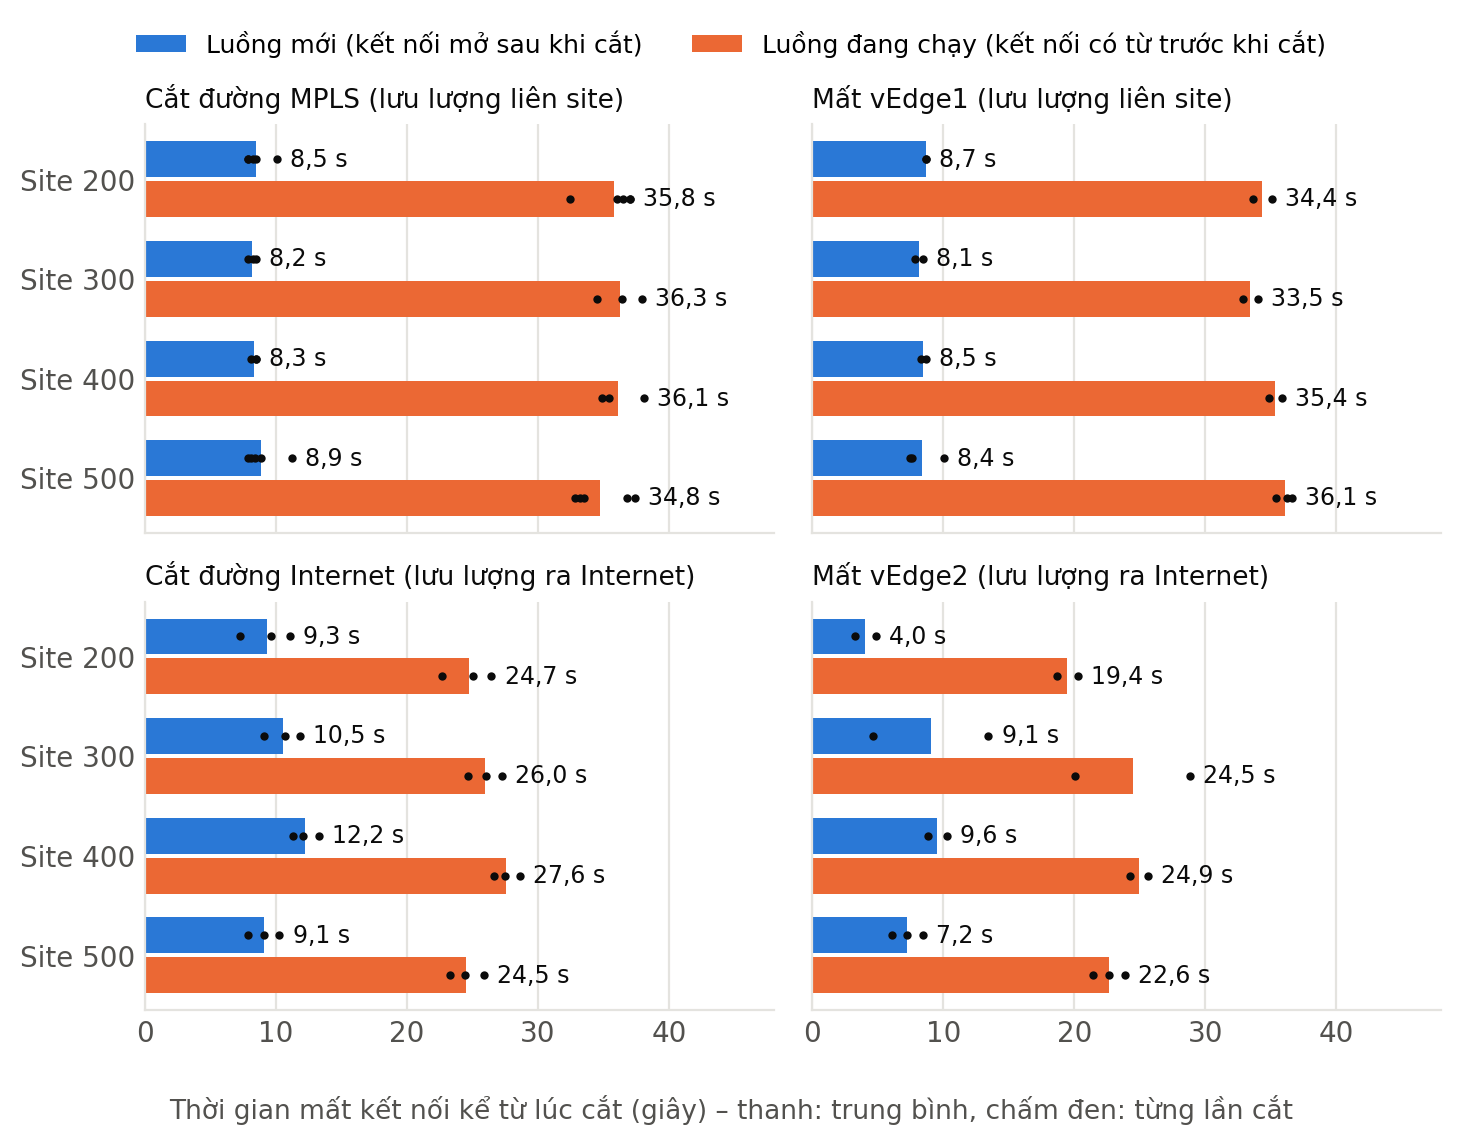
\includegraphics[width=\linewidth]{bd-failover-4site.png}
            \capt{Thời gian mất kết nối trung bình theo site và kịch bản}
        \end{column}
        \begin{column}{0.54\textwidth}
            \begin{columns}[T]
                \begin{column}{0.5\linewidth}\stat{brand}{3,2--13,4 s}{luồng mới tự khôi phục, cả 4 chi nhánh}\end{column}
                \begin{column}{0.5\linewidth}\stat{accent}{18,6--38,1 s}{luồng đang chạy (chờ \texttt{floating-conn})}\end{column}
            \end{columns}
            \begin{card}{Cơ chế}
                \scriptsize
                \begin{itemize}\compactlist
                    \item Brand-FW theo dõi \textbf{beacon} \texttt{10.1.255.1} bằng \texttt{sla monitor}/\texttt{track}; mất MPLS hoặc vEdge1 $\Rightarrow$ chuyển sang vEdge2.
                    \item Mất Internet hoặc vEdge2 $\Rightarrow$ ra Internet qua MPLS; nối lại thì tự quay về.
                    \item Không có beacon: chi nhánh \textbf{mất 100\,\% và không tự phục hồi}.
                \end{itemize}
            \end{card}
            \begin{softcard}[accentSoft]\scriptsize
                \textbf{Phép đo phát hiện 2 lỗi:} ASA ghim kết nối vào đường cũ (thêm \texttt{timeout floating-conn}); Site 500 thiếu \texttt{nat} trên cổng MPLS.
            \end{softcard}
        \end{column}
    \end{columns}
\end{frame}

\begin{frame}{SD-WAN -- failover tại Site 100, mất controller và AAR}
    \begin{columns}[T]
        \begin{column}{0.56\textwidth}
            \scriptsize
            \renewcommand{\arraystretch}{1.12}
            \rowcolors{2}{paper}{white}
            \begin{tabularx}{\linewidth}{@{}L{0.37\linewidth}YY@{}}
                \toprule
                \hd{Kịch bản tại Site 100} & \hd{Trước khi sửa} & \hd{Sau khi sửa (luồng mới)} \\
                \midrule
                Cắt một transport của vEdge1 & 7,6--8,6\,s & 8,6--9,2\,s \\
                Cắt cả hai transport của vEdge1 & Mất suốt thời gian cắt & \textbf{8,4--9,8\,s} \\
                Mất hẳn vEdge1 & Mất suốt thời gian cắt & \textbf{12,2--14,4\,s} \\
                Mất hẳn vEdge2 & Không mất gói & Không mất gói \\
                Internet khi mất vEdge1 & Mất suốt thời gian cắt & \textbf{3,6--7,6\,s} \\
                \bottomrule
            \end{tabularx}
            \vspace{0.1cm}
            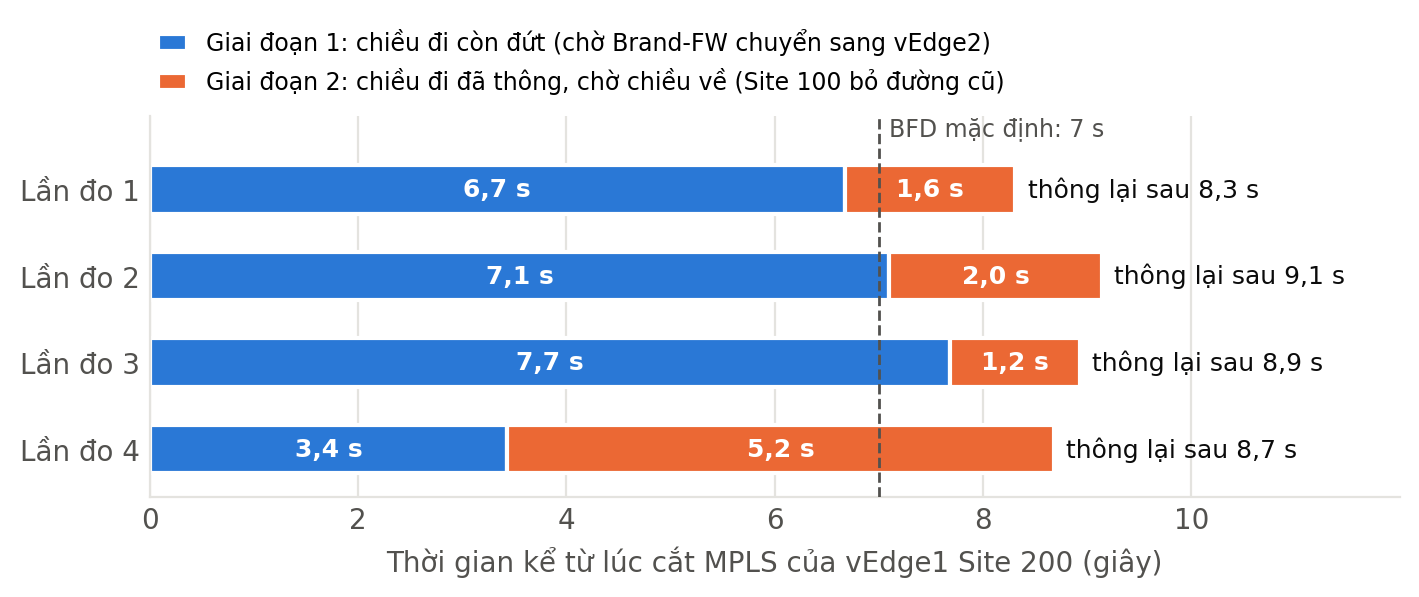
\includegraphics[width=0.62\linewidth]{bd-failover-2chieu.png}
            \capt{Hai giai đoạn khôi phục: chờ chiều đi (SLA), rồi chờ chiều về (BFD 7\,s)}
        \end{column}
        \begin{column}{0.42\textwidth}
            \begin{card}[okGreen]{Mất từng controller (2 phút)}
                \scriptsize
                Tắt vSmart, vBond, vManage 7 lần: \textbf{0 gói mất} trên overlay (0/22.500, 0/22.500, 0/15.000); kết nối lại sau 182--203\,s kể từ khi bật.
            \end{card}
            \begin{card}[accent]{AAR khi đường truyền suy giảm}
                \scriptsize
                Tăng trễ MPLS 400\,ms: lưu lượng tự chuyển sang \texttt{biz-internet} sau 5,5--7 phút, chỉ mất \textbf{4/7578 gói (0,05\,\%)}; gỡ thì tự quay về.
            \end{card}
            \begin{softcard}\scriptsize
                \textbf{Sửa lỗi thiết kế:} vEdge phân phối OMP vào OSPF (metric 10/100); tường lửa thêm SLA/\texttt{track}.
                AAR êm nhưng chậm $\Rightarrow$ đứt hẳn vẫn dựa vào BFD và \texttt{track}.
            \end{softcard}
        \end{column}
    \end{columns}
\end{frame}

\begin{frame}{Truy cập Internet tại chỗ (DIA) và cảnh báo email}
    \begin{columns}[c]
        \begin{column}{0.36\textwidth}
            \centering
            \shot{dia-brandfw-s200.png}
            \capt{Brand-FW Site 200: track, tuyến mặc định qua vEdge2, traceroute}
        \end{column}
        \begin{column}{0.62\textwidth}
            \scriptsize
            \renewcommand{\arraystretch}{1.1}
            \rowcolors{2}{paper}{white}
            \begin{tabularx}{\linewidth}{@{}L{0.46\linewidth}Y@{}}
                \toprule
                \hd{Kiểm thử} & \hd{Kết quả} \\
                \midrule
                Máy trạm Site 200/300/400: \texttt{ping google.com} & Đạt 3/3 mỗi site \\
                Traceroute từ chi nhánh ra Internet & Chặng đầu là vEdge2 tại chỗ, không vòng qua Site 100 \\
                Cắt \texttt{biz-internet} Site 200 rồi khôi phục & Chuyển sang MPLS, nối lại thì quay về \\
                VLAN 10 / VLAN 99 ra Internet & Thông / bị chặn đúng thiết kế \\
                Site 900 ra Internet có kiểm soát & DNS, HTTPS qua; HTTP 80, SSH 22 bị chặn \\
                \bottomrule
            \end{tabularx}
            \vspace{0.1cm}
            \begin{card}[accent]{Cảnh báo email từ vManage (tắt cổng Internet vEdge2 Site 200)}
                \scriptsize
                $\approx$20\,s: BFD down \,·\, $\approx$35\,s: Control down \,·\, $\approx$70\,s: OMP down \,·\, bật lại: Interface State Change --
                quản trị viên nhận cả thư \textbf{báo lỗi} lẫn thư \textbf{phục hồi}.
            \end{card}
            \begin{softcard}\scriptsize
                Lỗi đã xử lý: vEdge quảng bá ngược default làm nhà cung cấp mất Internet $\Rightarrow$ prefix-list \texttt{NO\_DEFAULT\_IN}.
            \end{softcard}
        \end{column}
    \end{columns}
\end{frame}

\begin{frame}{Dịch vụ -- DHCP và DNS tập trung}
    \begin{columns}[T]
        \begin{column}{0.30\textwidth}\centering
            \shot{dhcp-scopes-20261108.png}
            \capt{Bốn scope VLAN 10--40 đang hoạt động}
        \end{column}
        \begin{column}{0.30\textwidth}\centering
            \shot{dhcp-leases-vlan10-20261108.png}
            \capt{Lease VLAN 10 cấp qua DHCP Relay của Core}
        \end{column}
        \begin{column}{0.30\textwidth}\centering
            \shot{dns-zone-20261108.png}
            \capt{Zone \texttt{campus.internal}: MX và các bản ghi A}
        \end{column}
    \end{columns}
    \vspace{0.05cm}
    \begin{columns}[T]
        \begin{column}{0.49\textwidth}
            \begin{card}{Kết quả}
                \scriptsize
                \begin{itemize}\compactlist
                    \item Campus chính: 7/7 VPCS và máy Ubuntu nhận lease qua relay (\texttt{giaddr} .2/.3 chọn đúng scope).
                    \item Chi nhánh: 12/12 máy nhận đúng subnet, gateway, DNS \texttt{10.1.90.10}, tên miền.
                \end{itemize}
            \end{card}
        \end{column}
        \begin{column}{0.49\textwidth}
            \begin{card}[accent]{Bài học: tên miền \texttt{.local}}
                \scriptsize
                Máy Ubuntu chuyển \texttt{*.local} cho mDNS nên trình duyệt không tìm thấy máy chủ $\Rightarrow$ đổi toàn hệ thống sang \texttt{campus.internal}.
            \end{card}
        \end{column}
    \end{columns}
\end{frame}

\begin{frame}{Dịch vụ -- Web, Mail và Syslog từ mọi cơ sở}
    \begin{columns}[T]
        \begin{column}{0.30\textwidth}\centering
            \shot{web-campus-s100-20261108.png}
            \capt{\texttt{https://www.campus.internal} từ VLAN 40}
        \end{column}
        \begin{column}{0.30\textwidth}\centering
            \shot{mail-sent-s100-20261108.png}
            \capt{Thunderbird gửi thư qua SMTP 587}
        \end{column}
        \begin{column}{0.30\textwidth}\centering
            \shot{syslog-kiwi-20261108.png}
            \capt{Kiwi Syslog nhận nhật ký tường lửa, Web Server}
        \end{column}
    \end{columns}
    \vspace{0.05cm}
    \begin{columns}[T]
        \begin{column}{0.49\textwidth}
            \begin{card}{Từ chi nhánh Cần Thơ (qua overlay + tường lửa biên)}
                \scriptsize
                \begin{itemize}\compactlist
                    \item \texttt{/whoami} trả \texttt{client=10.2.70.103}: đi thẳng qua overlay, \textbf{không bị NAT}.
                    \item Gửi thư SMTP 587, đọc IMAP thành công; cổng 8080 bị chặn.
                \end{itemize}
            \end{card}
        \end{column}
        \begin{column}{0.49\textwidth}
            \begin{card}[accent]{Bài học: giới hạn ASAv không giấy phép}
                \scriptsize
                Tối đa 100 kết nối: truy vấn DNS ra ngoài chiếm đầy bảng làm IMAP bị từ chối dù ping vẫn thông
                $\Rightarrow$ ACL chỉ cho máy chủ DNS hỏi ra ngoài, giảm timeout DNS còn 10\,s.
            \end{card}
        \end{column}
    \end{columns}
\end{frame}

\begin{frame}{Vận hành tự động -- Campus NetOps Bot}
    \begin{columns}[T]
        \begin{column}{0.50\textwidth}
            \centering
            \begin{tikzpicture}[
                box/.style={draw=line, fill=white, rounded corners=3pt, align=center,
                            font=\scriptsize, minimum height=0.75cm, text width=2.3cm},
                bot/.style={box, draw=brand, fill=brandSoft, line width=0.8pt, text width=3.0cm, minimum height=1.1cm},
                arr/.style={-{Stealth[length=4pt]}, thick, brand}]
                \node[box, draw=accent] (tg) {Quản trị viên\\Telegram};
                \node[bot, below=0.4cm of tg] (bot) {\textbf{NetOps Bot}\\LangGraph + LLM\\(Server Farm Site 100)};
                \node[box, below left=0.55cm and -0.9cm of bot] (s100) {Site 100\\Core, FW-ASAv\\(SSH in-band)};
                \node[box, below right=0.55cm and -0.9cm of bot] (br) {Chi nhánh\\Brand-FW, switch\\(SSH qua SD-WAN)};
                \node[box, left=0.3cm of bot, text width=1.4cm] (vm) {vManage\\REST API};
                \node[box, right=0.3cm of bot, text width=1.4cm] (ryu) {Ryu\\REST API};
                \draw[arr, accent, <->] (tg) -- (bot);
                \draw[arr] (bot) -- (s100);
                \draw[arr] (bot) -- (br);
                \draw[arr] (bot) -- (vm);
                \draw[arr] (bot) -- (ryu);
            \end{tikzpicture}
        \end{column}
        \begin{column}{0.48\textwidth}
            \begin{card}{Bốn nhóm chức năng}
                \scriptsize
                \begin{itemize}\compactlist
                    \item \textbf{Hỏi đáp, lệnh chỉ đọc:} ngôn ngữ tự nhiên hoặc \texttt{/health}, \texttt{/show}, \texttt{/ping}, \texttt{/dhcp}.
                    \item \textbf{Chẩn đoán theo lớp} \texttt{/diag}: dừng ở lớp lỗi đầu tiên, kèm bằng chứng.
                    \item \textbf{Cảnh báo chủ động:} alarm vManage, OVS mất Controller; báo cả khi vManage hỏng.
                    \item \textbf{Thay đổi có duyệt} \texttt{/change}: tự hoàn tác nếu trạng thái xấu đi; \texttt{/compliance}, \texttt{/backup}, \texttt{/drift}.
                \end{itemize}
            \end{card}
            \begin{softcard}[okSoft]\scriptsize
                \textbf{\color{okGreen}An toàn:} chỉ chat được phép; tài khoản \texttt{netops} riêng, SSH chỉ từ 2 IP quản trị; che mật khẩu trong kết quả.
                Tự kiểm tra \textbf{23/23} mục.
            \end{softcard}
        \end{column}
    \end{columns}
\end{frame}

\begin{frame}{Campus NetOps Bot -- chạy thật trên Telegram}
    \begin{columns}[T]
        \begin{column}{0.30\textwidth}
            \centering
            {\scriptsize\textbf{\color{brand}\texttt{/health}} -- SD-WAN + SDN}\\[2pt]
            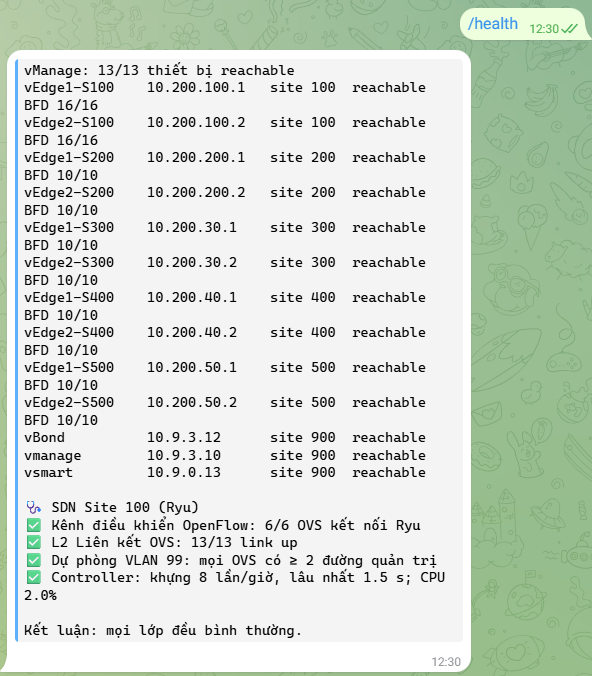
\includegraphics[height=0.52\textheight]{bot_health.png}
        \end{column}
        \begin{column}{0.34\textwidth}
            \centering
            {\scriptsize\textbf{\color{brand}\texttt{/diag fw}} -- tường lửa HA}\\[2pt]
            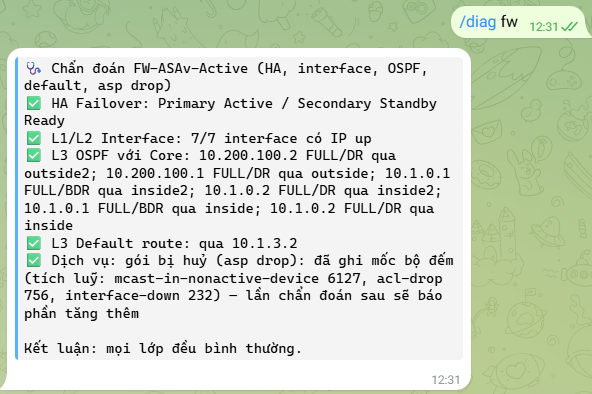
\includegraphics[width=0.84\linewidth]{bot_diag_fw.png}\\[3pt]
            {\scriptsize\textbf{\color{brand}\texttt{/diag site 200}} -- chi nhánh}\\[2pt]
            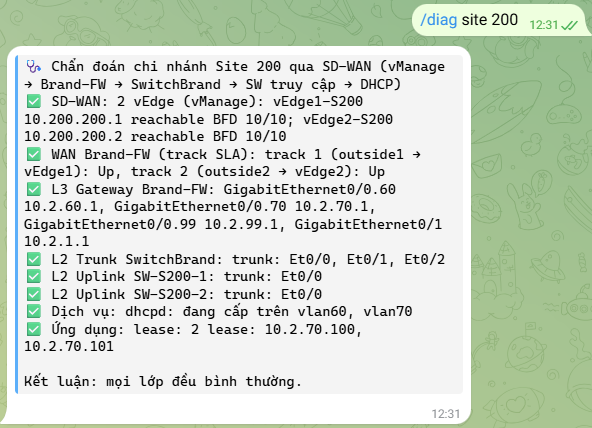
\includegraphics[width=0.74\linewidth]{bot_diag_site200.png}
        \end{column}
        \begin{column}{0.34\textwidth}
            \centering
            {\scriptsize\textbf{\color{accent}Hỏi tự nhiên} -- AI agent tự SSH}\\[2pt]
            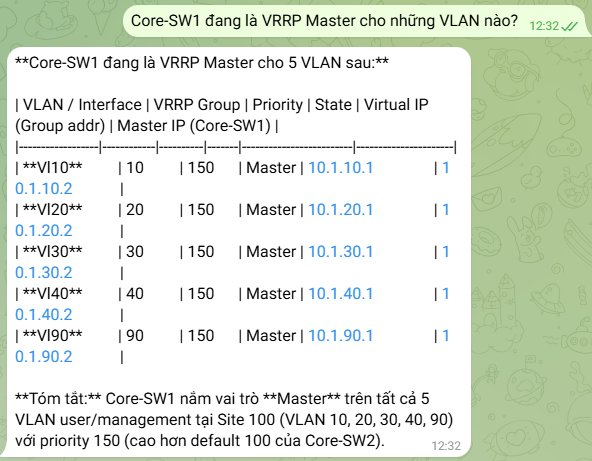
\includegraphics[width=\linewidth]{bot_ai_vrrp.png}
            \begin{softcard}\scriptsize
                13/13 thiết bị SD-WAN reachable, 6/6 OVS; FW Active/Standby Ready, 6 láng giềng OSPF FULL.
                Trong sự cố 01/11, cảnh báo của bot giúp tìm ra cặp tường lửa khởi động lại lặp.
            \end{softcard}
        \end{column}
    \end{columns}
\end{frame}

% ============================================================
% 05. ĐÁNH GIÁ VÀ KẾT LUẬN
% ============================================================
\section{Đánh giá và kết luận}

\begin{frame}{Tổng hợp 30 kịch bản kiểm thử}
    \begin{columns}[T]
        \begin{column}{0.76\textwidth}
            \scriptsize
            \renewcommand{\arraystretch}{1.16}
            \rowcolors{2}{paper}{white}
            \begin{tabularx}{\linewidth}{@{}L{0.22\linewidth}L{0.10\linewidth}Yc@{}}
                \toprule
                \hd{Nhóm} & \hd{Mã} & \hd{Bằng chứng chính} & \\
                \midrule
                Hạ tầng Campus chính & T01--T05 & 74 node, 107 mạng; VRRP 5/5 VLAN; FW HA dưới 1\,s đến 21\,s; DHCP Campus và chi nhánh & \pass \\
                SDN & T06--T12 & 6/6 switch, 13/13 liên kết; không bão; thêm VLAN 3,8\,ms; S1--S6 đạt; 0\,\% mất gói; chính sách 8,0--12,6\,ms & \pass \\
                SD-WAN & T13--T20 & BGP Established; 10 vEdge, 112 đường hầm; AAR, data/control policy 10/10; failover 3,2--14,4\,s & \pass \\
                Internet, cảnh báo & T21--T24 & DIA mọi site; dự phòng qua MPLS; chính sách theo vùng; thư BFD/Control/OMP & \pass \\
                Dịch vụ, bảo mật & T25--T28 & DNS, Web, Mail từ chi nhánh và Campus; ACL biên chặn 8080; Syslog UDP 514 & \pass \\
                Mở rộng, vận hành & T29--T30 & Site 500 vào fabric, RTT trung vị 4--7\,ms; NetOps Bot tự kiểm tra 23/23 & \pass \\
                \bottomrule
            \end{tabularx}
        \end{column}
        \begin{column}{0.22\textwidth}
            \stat{okGreen}{30/30}{kịch bản đạt}
            \stat{brand}{5/5}{nội dung đề cương đã hiện thực và kiểm chứng}
        \end{column}
    \end{columns}
    \vspace{0.05cm}
    \begin{softcard}\scriptsize
        Bốn kịch bản T10, T12, T22, T29 chỉ đạt sau khi đo đầy đủ dưới tải cao, tại mọi chi nhánh và \textbf{sửa các lỗi do chính phép đo phát hiện}.
    \end{softcard}
\end{frame}

\begin{frame}{Đối chiếu tiêu chí đề cương (1/2)}
    \vspace{0.05cm}
    \scriptsize
    \renewcommand{\arraystretch}{1.36}
    \rowcolors{2}{paper}{white}
    \begin{tabularx}{\textwidth}{@{}L{0.13\textwidth}L{0.19\textwidth}Y@{}}
        \toprule
        \hd{Nhóm} & \hd{Tiêu chí} & \hd{Kết quả đo} \\
        \midrule
        1. Hiệu năng & Throughput & 1,2\,Gbit/s cùng Access; 170\,Mbit/s liên VLAN; $\approx$2\,Mbit/s liên site (giới hạn WAN mô phỏng) \\
         & Delay, Jitter & LAN 0,43 / 1,57\,ms, jitter dưới 0,4\,ms; liên site RTT trung vị 4--7\,ms \\
         & Packet Loss & LAN 0\,\% (490/490); liên site 0\,\% (1500 gói) \\
        2. Mở rộng & Thời gian thêm VLAN & 3,8\,ms phần SDN; 5,3\,s gồm hai Core; dùng được sau $\approx$40\,s \\
         & Thời gian thêm Site & Nạp cấu hình vEdge $\approx$10\,s; site thông đầu--cuối sau 194--204\,s kể từ lúc bật nguồn \\
         & Số lệnh CLI & Một lệnh API cho 6 OVS, so với 18 lệnh CLI trên mỗi Core \\
        3. Độ tin cậy & Link Failover Time & SDN $\le$3,6\,s; chi nhánh 3,2--13,4\,s; Site 100 7,6--14,4\,s; FW HA dưới 1 đến 21\,s \\
         & Controller Recovery & Ryu: 6 switch nối lại sau $\approx$15\,s; SD-WAN: 182--203\,s, không mất gói dữ liệu \\
         & Packet Recovery Rate & 83,3--97,3\,\% (luồng mới), 48,8--87,1\,\% (luồng đang chạy) trên cả cửa sổ đo \\
         & Availability & 112 đường hầm: \textbf{99,957\,\%} trong 111,8 giờ; cả 5 site 100\,\% \\
        \bottomrule
    \end{tabularx}
\end{frame}

\begin{frame}{Đối chiếu tiêu chí đề cương (2/2)}
    \vspace{0.05cm}
    \scriptsize
    \renewcommand{\arraystretch}{1.36}
    \rowcolors{2}{paper}{white}
    \begin{tabularx}{\textwidth}{@{}L{0.13\textwidth}L{0.19\textwidth}Y@{}}
        \toprule
        \hd{Nhóm} & \hd{Tiêu chí} & \hd{Kết quả đo} \\
        \midrule
        4. Quản trị & Tự động hóa & VLAN, chính sách SDN: một lệnh API; chính sách SD-WAN khai một lần trên vSmart; NetOps Bot thay đổi có duyệt, tự hoàn tác \\
         & Xử lý sự cố & 4 sự cố gây chủ đích: chỉ ra lớp lỗi sau 0,1--7\,s, xác nhận phục hồi sau 3--17\,s \\
        5. Bảo mật & VLAN Isolation & Flood chỉ trong đúng VLAN; luật chặn VLAN 10 -- 40 chặn 5/5 gói, VLAN khác không ảnh hưởng \\
         & ACL Efficiency & ACL biên chặn cổng không công bố; data policy chặn Telnet/SSH, bộ đếm tăng đúng \\
         & Policy Enforcement & SDN: 8,0--12,6\,ms; SD-WAN: 4,4--5,0\,s kể từ lệnh commit trên vSmart \\
        6. QoS & SLA Satisfaction & 200,8 giờ: 96,3\,\% bản ghi thỏa SLA\_REALTIME, 98,2\,\% thỏa SLA\_BUSINESS; mọi cặp site luôn có đường hầm thỏa \\
         & VoIP MOS & $\approx$4,4 (ước lượng E-model); chất lượng video không đo được \\
         & Bandwidth Utilization & LAN 0,3\,\% khi rảnh, 9,8--93\,\% ở 10--100\,Mbit/s; WAN bão hòa ở 2\,Mbit/s \\
        7. Quy mô & Switch, Host, Branch & 6 OVS + 18 switch Cisco; 22 máy trạm; 4 cơ sở phụ; 10 vEdge \\
         & CPU, RAM Controller & Ryu 4--9\,\% CPU khi rảnh, 41,3\,\% ở 1000 MAC mới/giây, 944\,MB RAM \\
        \bottomrule
    \end{tabularx}
\end{frame}

\begin{frame}{Các phép đo theo tiêu chí vận hành}
    \begin{columns}[T]
        \begin{column}{0.235\textwidth}\stat{brand}{194--204 s}{thêm site: bật nguồn đến thông đầu--cuối}\end{column}
        \begin{column}{0.235\textwidth}\stat{accent}{4,4--5,0 s}{chính sách SD-WAN có hiệu lực tại vEdge}\end{column}
        \begin{column}{0.235\textwidth}\stat{okGreen}{96,3 \%}{thỏa SLA\_REALTIME trong 200,8 giờ}\end{column}
        \begin{column}{0.235\textwidth}\stat{brand}{99,957 \%}{độ khả dụng 112 đường hầm}\end{column}
    \end{columns}
    \vspace{-0.1cm}
    \scriptsize
    \renewcommand{\arraystretch}{1.12}
    \rowcolors{2}{paper}{white}
    \begin{tabularx}{\textwidth}{@{}L{0.31\textwidth}L{0.17\textwidth}YL{0.08\textwidth}L{0.14\textwidth}@{}}
        \toprule
        \hd{Sự cố gây chủ đích (3 lần mỗi loại)} & \hd{Phát hiện} & \hd{Chẩn đoán theo lớp (NetOps Bot)} & \hd{Sửa} & \hd{Phục hồi} \\
        \midrule
        Đứt uplink Access-SW1 -- Dist-SW1 & 1,7--2,3\,s (Controller) & 0,1\,s; đúng lớp liên kết OVS & $<$0,1\,s & 3,1\,s \\
        Đứt đường MPLS của vEdge1 Site 200 & 17,2--22,5\,s (alarm) & 6,5--7,0\,s; dừng ở lớp kết nối điều khiển & $<$0,1\,s & 7,2--16,7\,s \\
        Shutdown cổng SwitchBrand Site 200 & Không có cảnh báo & 5,2\,s; đúng lớp trunk SwitchBrand & 0,3\,s & 12,4--13,3\,s \\
        Mất \texttt{ip helper-address} trên Core-SW1 & Không có cảnh báo & 3,0\,s; đúng lớp DHCP relay & 0,3\,s & 4,7--5,3\,s \\
        \bottomrule
    \end{tabularx}
    \vspace{0.05cm}
    {\scriptsize\color{inkSoft}Số đo là phần việc của công cụ, không tính phản ứng của người vận hành; thêm site chưa gồm bước ký chứng chỉ; tỷ lệ thỏa SLA là cận dưới.\par}
\end{frame}

\begin{frame}{So sánh với các mô hình đối chứng}
    \vspace{0.05cm}
    \scriptsize
    \renewcommand{\arraystretch}{1.08}
    \rowcolors{2}{paper}{white}
    \begin{tabularx}{\textwidth}{@{}L{0.13\textwidth}L{0.17\textwidth}L{0.19\textwidth}L{0.19\textwidth}Y@{}}
        \toprule
        \hd{Tiêu chí} & \hd{Flat, Two-Tier} & \hd{Three-Tier truyền thống} & \hd{VXLAN EVPN} & \hd{\color{brand}Đề xuất (SDN + SD-WAN)} \\
        \midrule
        Chống vòng, hội tụ L2 & STP 30--50\,s; RSTP vài giây & RSTP vài giây, chặn cổng dư & Không cần STP trong fabric, ECMP & \textbf{Đo:} hội tụ dưới 16\,ms, gián đoạn $\le$3,6\,s \\
        Thêm VLAN & CLI từng switch & CLI từng switch và Core (\textbf{đo:} 18 lệnh mỗi Core) & Khai VNI trên các leaf & \textbf{Đo:} một lệnh API, 3,8\,ms cho 6 OVS \\
        Chính sách & Từng thiết bị & Từng thiết bị & Tập trung nếu có bộ điều khiển & \textbf{Đo:} 8,0--12,6\,ms; vSmart cho mọi chi nhánh \\
        Liên cơ sở & Một đường WAN, tuyến tĩnh & WAN truyền thống & Cần giải pháp liên site riêng & Overlay IPsec 2 transport, chọn đường theo SLA \\
        Failover WAN & Thủ công & Theo hội tụ định tuyến & Phụ thuộc underlay & \textbf{Đo:} 3,2--13,4\,s với luồng mới \\
        Điểm yếu & Không mở rộng, bão broadcast & Cấu hình thủ công, dễ lệch & Đòi hỏi thiết bị, kỹ năng cao & Controller là điểm trọng yếu; in-band phức tạp \\
        \bottomrule
    \end{tabularx}
    \vspace{0.08cm}
    \begin{softcard}\scriptsize
        So sánh \textbf{định tính}; chỉ số ghi ``Đo'' là của đề tài. Đối chứng đo trên hệ thống:
        kênh VLAN 99 phụ thuộc RSTP gián đoạn \textbf{10,9\,s} $\rightarrow$ Controller chống vòng \textbf{0\,s};
        chi nhánh đứt MPLS \textbf{không tự phục hồi} $\rightarrow$ nay \textbf{7,4--11,2\,s}.
    \end{softcard}
\end{frame}

\begin{frame}{Kết quả đạt được}
    \begin{columns}[T]
        \begin{column}{0.325\textwidth}
            \begin{card}{Hạ tầng và dịch vụ}
                \scriptsize
                \begin{itemize}\compactlist
                    \item Quy hoạch IP/VLAN/System-IP/ASN thống nhất theo mã site.
                    \item Hai kiến trúc cùng tồn tại: 3 tầng có SDN và Firewall-as-Core.
                    \item VRRP, OSPF, tường lửa HA tự chuyển vai trò (dưới 1\,s đến 21\,s).
                    \item DNS, Web, Mail, Syslog dùng được từ mọi cơ sở; Internet tại chỗ có dự phòng.
                \end{itemize}
            \end{card}
        \end{column}
        \begin{column}{0.325\textwidth}
            \begin{card}[accent]{SDN}
                \scriptsize
                \begin{itemize}\compactlist
                    \item Ứng dụng Ryu điều khiển toàn bộ lớp 2 của 6 OVS; Console 10 trang.
                    \item Thêm VLAN \textbf{3,8\,ms}; chính sách \textbf{8,0--12,6\,ms}; hội tụ dưới 16\,ms.
                    \item Gián đoạn $\le$\textbf{3,6\,s}; 6/6 kịch bản tự phục hồi đạt.
                    \item 1,2\,Gbit/s cùng Access; 1000 MAC mới/giây với 41\,\% CPU.
                \end{itemize}
            \end{card}
        \end{column}
        \begin{column}{0.325\textwidth}
            \begin{card}[okGreen]{SD-WAN và vận hành}
                \scriptsize
                \begin{itemize}\compactlist
                    \item 10 vEdge xác thực PKI, 112 đường hầm trên 2 transport.
                    \item SLA, AAR, data/control policy: \textbf{10/10} tại 4 chi nhánh.
                    \item 46 lần cắt thật: tự khôi phục \textbf{3,2--13,4\,s}; mất controller không mất gói.
                    \item NetOps Bot: chẩn đoán theo lớp, cảnh báo, thay đổi có duyệt.
                \end{itemize}
            \end{card}
        \end{column}
    \end{columns}
    \begin{softcard}[okSoft]\scriptsize
        \textbf{\color{okGreen}Về phương pháp:} triển khai từ dưới lên, chẩn đoán theo lớp, có bằng chứng cho từng kết luận
        $\Rightarrow$ tìm ra nguyên nhân gốc của nhiều sự cố không hiển nhiên (flow in-band ẩn của OVS, RSTP \textit{Dispute}, tuyến /24 che đường điều khiển, \texttt{.local} và mDNS).
    \end{softcard}
\end{frame}

\begin{frame}{Hạn chế và hướng phát triển}
    \begin{columns}[T]
        \begin{column}{0.49\textwidth}
            \begin{card}[badRed]{Hạn chế}
                \scriptsize
                \begin{itemize}\compactlist
                    \item \textbf{SDN Controller là điểm lỗi đơn}; khi máy chủ quá tải, Controller khựng tới 4\,s.
                    \item \textbf{Controller SD-WAN chưa dự phòng}: mất controller không mất gói nhưng không đổi được chính sách.
                    \item \textbf{Luồng đang chạy khôi phục chậm} (19--38\,s) do chờ \texttt{floating-conn}; timer BFD mặc định.
                    \item \textbf{Giới hạn mô phỏng:} WAN $\approx$2\,Mbit/s; ASAv không giấy phép $\approx$0,1\,Mbit/s, 100 kết nối.
                    \item 802.1X, DHCP Snooping, DAI, SNMPv3, AAA mới ở mức thiết kế.
                    \item Một số tiêu chí mới đo một phần (thêm site chưa gồm ký chứng chỉ; MOS là ước lượng); chính sách SD-WAN cấu hình bằng CLI trên vSmart.
                \end{itemize}
            \end{card}
        \end{column}
        \begin{column}{0.49\textwidth}
            \begin{card}[okGreen]{Hướng phát triển}
                \scriptsize
                \begin{enumerate}\compactlist
                    \item \textbf{Controller dự phòng nóng} (master/slave OpenFlow) hoặc nền tảng hỗ trợ cluster.
                    \item \textbf{Giảm thời gian failover:} timer BFD ngắn sau khi nâng vCPU, giảm chu kỳ SLA, OSPF graceful restart.
                    \item \textbf{Tăng cường bảo mật:} 802.1X, chống DHCP/ARP giả mạo bằng flow, SSH/SNMPv3, AAA tập trung.
                    \item \textbf{Chuẩn hóa SD-WAN} bằng template và chính sách trên vManage.
                    \item \textbf{Tự động hóa:} kiểm tra nhất quán thiết kế -- cấu hình; triển khai qua API (Ansible, vManage, Ryu).
                    \item \textbf{Đo kiểm trên thiết bị thật} để đối chiếu với môi trường ảo.
                \end{enumerate}
            \end{card}
        \end{column}
    \end{columns}
\end{frame}

\begin{frame}{Kết luận}
    \vspace{0.1cm}
    \begin{card}{SDN và SD-WAN kết hợp được trong một kiến trúc Campus đa cơ sở}
        \footnotesize
        \begin{itemize}\setlength{\itemsep}{3pt}
            \item \textbf{Cơ chế truyền thống vẫn giữ vai trò:} VRRP, OSPF, tường lửa HA và VLAN bảo đảm ổn định tại lớp 3 và biên mạng.
            \item \textbf{Ryu} mang lại khả năng lập trình, tự phục hồi và quan sát tập trung cho lớp 2, với thời gian thêm VLAN và áp chính sách tính bằng \textbf{mili giây}.
            \item \textbf{vManage, vSmart, vBond} điều phối overlay an toàn, chính sách tập trung, tự chọn đường giữa các cơ sở và chủ động cảnh báo.
        \end{itemize}
    \end{card}
    \begin{columns}[T]
        \begin{column}{0.49\textwidth}
            \begin{softcard}[accentSoft]\scriptsize
                \textbf{\color{accent}Thách thức thực tế của SDN in-band:} phụ thuộc vòng giữa switch và Controller, trách nhiệm chống vòng chuyển sang Controller, tương tác ngầm với STP.
            \end{softcard}
        \end{column}
        \begin{column}{0.49\textwidth}
            \begin{softcard}\scriptsize
                \textbf{\color{brand}Yêu cầu chặt chẽ của SD-WAN:} chứng thư, định tuyến tới controller cho từng màu TLOC, lọc tuyến tại nhà cung cấp.
            \end{softcard}
        \end{column}
    \end{columns}
    \vspace{0.05cm}
    {\centering\footnotesize\color{inkSoft}Mô hình có thể dùng làm nền tảng thực hành, nghiên cứu và thử nghiệm chính sách mạng Campus đa cơ sở.\par}
\end{frame}

% ============================================================
% KẾT THÚC
% ============================================================
{\setbeamertemplate{background}{}\setbeamertemplate{footline}{}
\begin{frame}[plain, noframenumbering]
    \begin{tikzpicture}[remember picture, overlay]
        \fill[navy] (current page.south west) rectangle (current page.north east);
        \fill[brand] ([xshift=-1.5cm, yshift=-0.6cm]current page.center) rectangle ([xshift=0.9cm, yshift=-0.66cm]current page.center);
        \fill[accent] ([xshift=0.9cm, yshift=-0.6cm]current page.center) rectangle ([xshift=1.5cm, yshift=-0.66cm]current page.center);
        \node[text=white, font=\huge\bfseries, align=center] at ([yshift=0.4cm]current page.center) {Cảm ơn quý thầy cô đã lắng nghe!};
        \node[text=white!70!navy, font=\small] at ([yshift=-1.2cm]current page.center) {Nhóm xin được lắng nghe câu hỏi và góp ý của hội đồng};
        \node[text=white!70!navy, font=\footnotesize] at ([yshift=-1.9cm]current page.center) {Trần Hữu Nhân \,·\, Nguyễn Nhật Hào};
    \end{tikzpicture}
\end{frame}}

\end{document}
